%%%%%%%%%%%%%%%%%%%%%%%%%%%%%%%%%%%%%%%%%%%%%%%%%%%%%%%%%%%%%
% This document can be formatted only with pdflatex.
%%%%%%%%%%%%%%%%%%%%%%%%%%%%%%%%%%%%%%%%%%%%%%%%%%%%%%%%%%%%%

\documentclass[12pt,twoside,a4paper]{article}
\usepackage[hyphens]{url}
\usepackage[bookmarks=true,hyperindex=true,colorlinks=true,linkcolor=blue,citecolor=blue,backref=page,pagebackref=true,plainpages=false,pdfpagelabels]{hyperref}
\usepackage{bookmark}

\usepackage[T1]{fontenc}
\usepackage{ae}
\usepackage[pdftex]{graphicx}
\graphicspath{{Figs/}}

\usepackage{Templates/LaTeX/togdoc}

\usepackage[english]{babel}
\usepackage{latexsym,epsf,epsfig}
\usepackage{rotating,amsmath,amsfonts,amssymb}
%\usepackage{subfigure}

\DeclareUnicodeCharacter{2019}{'}
\DeclareUnicodeCharacter{2018}{`}
\DeclareUnicodeCharacter{201C}{``}
\DeclareUnicodeCharacter{201D}{''}
\DeclareUnicodeCharacter{2013}{--}
\DeclareUnicodeCharacter{2014}{---}
\DeclareUnicodeCharacter{2026}{...}
\DeclareUnicodeCharacter{00A0}{~}
\DeclareUnicodeCharacter{2022}{-}   % bullet

\usepackage{times}
\usepackage{listings}
\usepackage{courier}
\usepackage{longtable}
\usepackage{pdfpages}
\usepackage{multirow}
\usepackage{booktabs}
\usepackage{datetime}
\usepackage{xcolor}

\usepackage{tabularx}

\usepackage{forest}
\usepackage{microtype}
\usepackage[export]{adjustbox}

\forestset{
  aco tree/.style={
    for tree={
      grow'=south,
      parent anchor=south,
      child anchor=north,
      align=left,
      rounded corners,
      inner sep=2pt,
      s sep=100pt,
      l sep=6pt,
      edge={-},
      font=\scriptsize,
      text width=.48\linewidth,
    }
  }
}

\definecolor{myRomanGreen}{RGB}{69, 139, 0}
\lstset{basicstyle=\footnotesize\ttfamily,breaklines=true}

\usepackage{xr}

\sloppy

%%%%%%%%%%%%%%%%%%%%%%%%%%%%%%%%%%%%%%%%%%%%%%%%%%%%%%%%%%%%%%%%%%%%%
% Change title and other document information here.                 %
%%%%%%%%%%%%%%%%%%%%%%%%%%%%%%%%%%%%%%%%%%%%%%%%%%%%%%%%%%%%%%%%%%%%%
\newcommand{\dnumber}{0}

\newcommand{\dtitle}{%
  Open Evidential Tool Bus\\(O-ETB) v1.1.4\\User Manual
}
%\newcommand{\dshorttitle}{O-ETB v1.1.3 User Manual}
\newcommand{\dshorttitle}{User Manual}
\newcommand{\dversion}{11}  % Document Version number
\newcommand{\dauthors}{The Open Group}
\newcommand{\dstatus}{Draft}
\newcommand{\ddist}{Public}

\newdateformat{eudate}{\THEDAY~\monthname[\THEMONTH]~\THEYEAR}
\newcommand{\ddate}{\eudate \today}
\newcommand{\dyear}{\the\year{} }

\renewcommand{\thefigure}{\arabic{figure}}

%\usepackage{fancyhdr}
%\usepackage{fancyvrb}
%\pagestyle{fancy}
\fancyhead[RO,LE]{\dshorttitle}
%\fancyhead[LO,RE]{The Open Group}
\fancyhead[LO,RE]{O-ETB v1.1.4}
%\cfoot{center}
%\fancyfoot[LO,RE]{\footnotesize \ddate}
%\fancyfoot[RO,LE]{\footnotesize\rm Page \thepage}
%%\fancyfoot[LO,RE]{\ddate}
\fancyfoot[RO,LE]{The Open Group}
%\fancyfoot[CO,CE]{Version \dversion}
\fancyfoot[CO,CE]{\rm \thepage}
\fancyfoot[LO,RE]{\rm Version \dversion}

%%%%%%%%%%%%%%%%%%%%%%%%%%%%%%%%%%%%%%%%%%%%%%%%%%
%% LOCAL CHANGES START %%
%%%%%%%%%%%%%%%%%%%%%%%%%%%%%%%%%%%%%%%%%%%%%%%%%%

\usepackage[colorinlistoftodos]{todonotes}
\usepackage{xr}
\usepackage{stmaryrd}
%\usepackage{mathpartir}
\usepackage{theorem}
\usepackage{verbatim}

\usepackage{colonequals}
\newcommand*{\logeq}{\ratio\Leftrightarrow}


\usepackage{titlesec}
\usepackage{hyperref}

\titleformat{\paragraph}
{\normalfont\normalsize\bfseries}{\theparagraph}{1em}{}
\titlespacing*{\paragraph}
{0pt}{3.25ex plus 1ex minus .2ex}{1.5ex plus .2ex}
\makeatletter
\renewcommand\paragraph{\@startsection{paragraph}{5}{\z@}%
  {3.25ex \@plus1ex \@minus.2ex}%
  {-1em}%
  {\normalfont\normalsize\bfseries}}
  \def\l@paragraph{\@dottedtocline{5}{7em}{5em}}
\def\toclevel@paragraph{5}
\makeatother

\setcounter{secnumdepth}{5}
\setcounter{tocdepth}{5}

% define external documents:
%\externaldocument[FVSreq:]{../../WP2/d2_1/d2_1}
% ... add more as needed

\allowdisplaybreaks

%
% Page layout
%
\renewcommand{\topfraction}{1.0}
\renewcommand{\bottomfraction}{1.0}
\renewcommand{\textfraction}{0.0}
\setcounter{topnumber}{4}

% inline red TODO text
\newcommand{\intodo}[1]{\textcolor{red}{\text{TODO: #1}}}

% Examples
{\theorembodyfont{\rmfamily}\newtheorem{example}{Example}}

%%%%%%%%%%%%%%%%%%%%%%%%%%%%%%%%%%%%%%%%%%%%%%%%%%
%% LOCAL CHANGES END %%
%%%%%%%%%%%%%%%%%%%%%%%%%%%%%%%%%%%%%%%%%%%%%%%%%%

\usepackage{multicol}
\usepackage{bytefield}
\usepackage{colortbl}
\usepackage{textcomp}

\usepackage{cite}

\newlength{\hsbw}
\newcommand{\memo}[1]{\mbox{}\par\vspace{0.25in}%
\setlength{\hsbw}{\linewidth}%
\addtolength{\hsbw}{-2\fboxsep}%
\addtolength{\hsbw}{-2\fboxrule}%
\noindent\fbox{\parbox{\hsbw}{{\bf Memo: }#1}}\vspace{0.25in}}

% comment-out next line to hide Memos
%\renewcommand{\memo}[1]{}



\begin{document}
\firstpage
\newpage
~

\newpage
\tableofcontents
\listoffigures
\listoftables
% % % % % % % % % % % % % % % % % % % % % % % % % % % % % % % % % % % % % % % %
\clearpage
\pagenumbering{arabic}

%%%%%%%%%%%%%%%%%%%%%%%%%%%%%%%%%%%%%%%%%%%%%%%%%%%%%%%%%%%%





\hypertarget{introduction}{%
\section{Introduction}\label{introduction}}

This User Manual version 10 for the Open Evidential Tool Bus (O-ETB) Version 1.1.3 represents revisions and additions of material actively ongoing. It is a living document with its own version number, as multiple versions of the User Manual may apply to the same version of O-ETB as identified in the title. Higher numbered versions of the User Manual supersede lower numbered versions.

ACKNOWLEDGMENTS:

The O-ETB is based on the Adaptive MILS Evidential Tool Bus (AM-ETB) from the EC CITADEL Project (Critical Infrastructure Protection Using Adaptive MILS, Project Number 700665), implemented by Marius Bozga of Université Grenoble Alpes, with reorganization and continuing development by Rance DeLong of The Open Group. Contributions to argument patterns and assurance tools and approaches were made by atsec information systems, University of York, Fondazione Bruno Kessler, Université Grenoble Alpes and other partners in the CITADEL and D-MILS EC projects.

\clearpage
\hypertarget{o-etb-assurance-tool-configurations}{%
\section{O-ETB Assurance Tool configurations}\label{o-etb-assurance-tool-configurations}}

The O-ETB Assurance Tool may be delivered in several configurations, representing different modes of access to common underlying functionalities, that provide for the construction of assurance cases, along with their supporting evidence, in a form appropriate for evaluation by other parties such as certifiers.

The current configuration of the Assurance Tool provides a command-based interface that can be used interactively and/or in a batch mode to execute single commands or to run pre-defined command scripts or user defined command scripts.

A possible future Assurance Server configuration would provide programmatic access to the core functions of the Assurance Tool through an API. Though not currently implemented, this manual contains comments concerning potential features and properties of such a server.

All configurations run on a shared common file structure defined by O-ETB, or, for development, testing or experimentation, on independent instances of the same file structure, as determined by configuration options and invocation arguments. As part of that file structure, assurance cases and evidence are constructed and updated incrementally and stored persistently in the CASES and EVIDENCE Repositories respectively.

The core workflow of O-ETB utilises \emph{tool agents} to incorporate external evidence-generating tools into the workflow and to store their results in a canonical form into the EVIDENCE Repository.

Tool agents serve as adaptors to include external evidence-producing tools into the O-ETB core workflow and their results into the EVIDENCE Repository. A tool agent embodies knowledge about the data that is required for successful running of a tool, about executing the tool, about interpreting the results of executing the tool, and about reporting the results back to the ETB core workflow through a protocol that includes a combination of tool agent return codes and direct manipulation of files in the EVIDENCE Repository.

O-ETB includes rendering functions that use information from the Repository to create collections of artefacts for certification efforts according to requirements of a particular target certification domain.

\hypertarget{o-etb-git-repository-organisation}{%
\subsection{O-ETB Git repository organisation}\label{o-etb-git-repository-organisation}}

The O-ETB Git repository structure, available on GitHub at MedSecurance/Assurance and tog-rtd/O-ETB, consolidates development directories and database directories.
Development directores contain source code, documentation and other artefacts relating to design, development, testing and deployment.
Database directories are relevant to configuraiton and runtime operation.

source code with new directory structure elements for dynamic data resources including a knowledge base, repositories for changeable persistent data comprising assurance cases and assurance evidence, artefact collections comprising certification assurance packages, build space, and documents. Figure~\ref{fig:top-repo} shows the top-level structure of the O-ETB source repository. This includes subdirectories related to both development, including src, doc, BUILD and TEST, and subdirectories the hold the runtime and persistent data structures, including KB, REPOSITORY and CAP. Annex A contains a complete list of files in the O-ETB source repository.


\protect\hypertarget{_Ref168316389}{}{}
\begin{figure}[htbp]
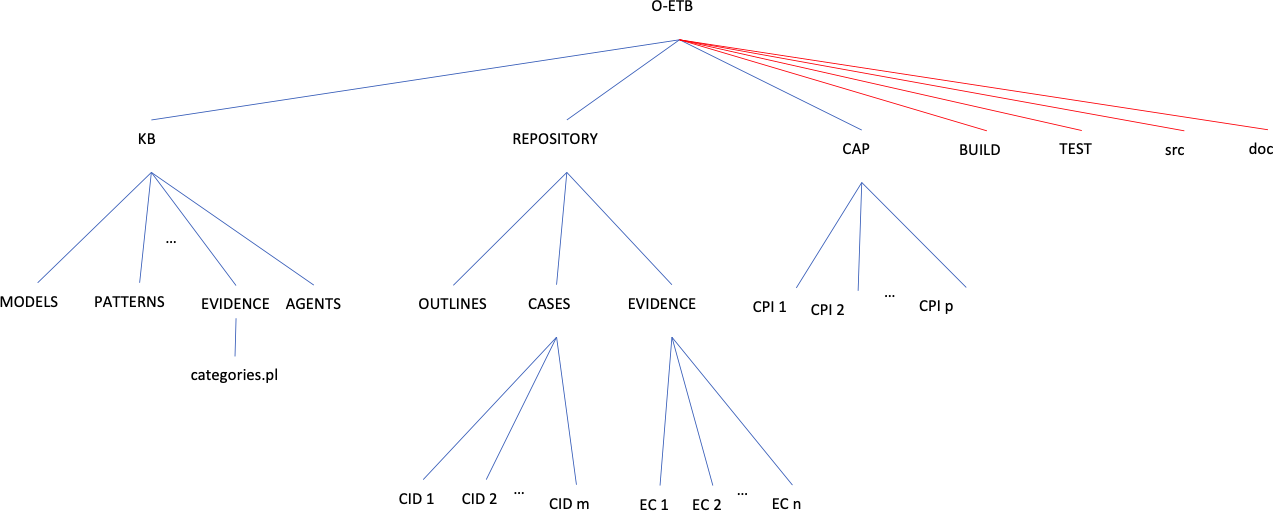
\includegraphics[width=6.5in,height=2.125in]{figures/O-ETB-Final-Git-Repo}
\caption{O-ETB Git repository top-level structure}\label{fig:top-repo} 
\end{figure}
\hypertarget{_Ref165897405}{}{}


\hypertarget{development-directories}{%
\subsubsection{Development directories}\label{development-directories}}

These directories contain the implementation source code, tests, build and deployment workspace and documentation for O-ETB.

\hypertarget{src-directory}{%
\paragraph{src directory}\label{src-directory}}

The Prolog source code, including declaration of static and dynamic predicates, has been consolidated into a ``src'' sub-directory of the O-ETB source repository.
This directory and subdirectories contain the source code modules comprising O-ETB.

In the present evolution module files have been added for functionalities such as a command line interpreter, command-invoked actions, command procedures and scripts, self-tests, and parameterization of the implementation.

The source code organization has been enhanced by moving user modifiable source configuration data to the Knowledge Base and by the addition of a global parameters file (``param.pl'') that consolidates O-ETB operational settings and constant definitions in one place from where the parameters are referenced at appropriate places in the source code.

Annex A presents the complete list of source code files and modules in O-ETB v1.1.3.


\hypertarget{docs-directory}{%
\paragraph{docs directory}\label{docs-directory}}

This directory contains README files as well as this User Manual, Release Note, Assurance Glossary (described further in Annex E), argument patterns document, Assurance Case Outline (ACO) specification, ACO Quick Reference Card and design documents and diagrams.

\hypertarget{build-directory}{%
\paragraph{BUILD directory}\label{build-directory}}

The BUILD directory contains the etb and etb-server executables built by the makefile residing in the src directory. It also contains other files related to build and deployment of O-ETB.
Since the etb executable references the TEST, KB, REPOSITORY and CAP directories with a prefix of '../', etb should be run either from BUILD (if running the pro-compiled version) or from the src directory (if loading and running from source).

\hypertarget{test-directory}{%
\paragraph{TEST directory}\label{test-directory}}

This directory contains O-ETB test cases, and in the future will contain more test cases, regression test scripts, and test results.


\hypertarget{database-directories}{%
\subsubsection{Database directories}\label{database-directories}}

These directories contain the data structures that represent the persistent but mutable state of an O-ETB database instance. These contain target-of-assurance information and derived artefacts for potentially multiple assurance and certification efforts that share a common (but dynamic) knowledge base.

Figure~\ref{fig:db-repo} illustrates the structure of the database portion of the O-ETB source repository.


\begin{figure}[htbp]
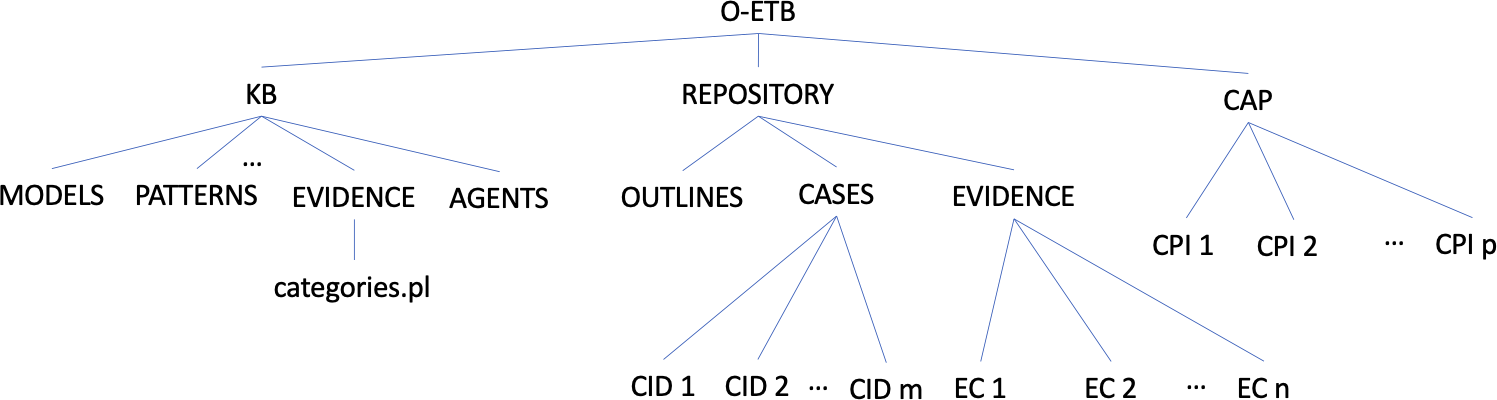
\includegraphics[width=6.5in,height=2.125in]{figures/O-ETB-Final-DB.pdf}
\caption{Database structure}\label{fig:db-repo} 
\end{figure}


\hypertarget{KB-directory}{%
\paragraph{Knowledge Base (KB) directory}\label{KB-directory}}

A distinct place in the runtime file structure has been created for the knowledge base used by O-ETB (``KB'' directory). The knowledge base includes the library of assurance case argument patterns (``PATTERNS'' sub-directory), the library of system models (``MODELS'' sub-directory), a library of workflow patterns (``WORKFLOWS'' sub-directory), and in the future will be extended with other directories for additional expert knowledge applicable to the construction of assurance cases, evidence categories with corresponding evidential tools, and specifications for the requirements on the content and presentation for certification assurance packages.


\hypertarget{REPO-directory}{%
\paragraph{REPOSITORY directory}\label{REPO-directory}}

The repository is where O-ETB stores internal representations of artefacts comprising aspects of assurance cases under construction.
Specifically, there are branches for assurance case outlines (OUTLINES), instantiated assurance cases (CASES) and evidence records and status (EVIDENCE).



\hypertarget{CAP-directory}{%
\paragraph{Certification Assurance Package (CAP) directory}\label{CAP-directory}}

The CAP directory is the place to which O-ETB exports assurance cases from the repository into forms suitable for browsing the results and making results available for further processing.



\hypertarget{assurance-case-and-evidence-repositories}{%
\subsubsection{Assurance outlines, case and evidence repositories}\label{assurance-case-and-evidence-repositories}}

Under the ``REPOSITORY'' directory the assurance outlines repository (``OUTLINES''), the assurance case repository (``CASES'' sub-directory) and the evidence repository (``EVIDENCE'' sub-directory) are located. Separate directories are created under CASES for each assurance case. The EVIDENCE directory is organized by directories corresponding to evidence categories and under those are sub-directories are used for individual evidence records.

\hypertarget{certification-assurance-package}{%
\subsubsection{Certification Assurance Package}\label{certification-assurance-package}}

The runtime file structure includes a default location (``CAP'' directory) for the export of collections of artefacts tailored to specific certification targets.

\hypertarget{etb-assurance-tool}{%
\subsection{`etb' Assurance Tool}\label{etb-assurance-tool}}

The `etb' tool enables AC pattern development, AC pattern instantiation and Assurance Tool development and testing. The etb tool provides the ability to test AC patterns under development and use of the knowledge base and tool agents.

\hypertarget{command-line-options}{%
\subsubsection{Command line options}\label{command-line-options}}

When a compiled version of the O-ETB Assurance Tool is started from the command line as ``etb'', several command line options are recognized. NEW

\begin{itemize}
\item
  -\/-command, -c \textless etb command\textgreater{} execute the specified command and exit. Note that this command could be proc or script, which will run a previously defined sequence of commands NEW
\item
  -\/-model, -m \textless model directory\textgreater{} load a model specification from the specified directory under KB/MODELS before the -\/-command, -c option is processed if it has been specified or before entering the interactive command interpreter. NEW
\item
  -\/-patterns, -p \textless patterns file name\textgreater{} load a user-provided patterns definition file. This option is processed before the -\/-command, -c option, or if that option has not been specified then before entering the interactive command interpreter. NEW
\item
  -\/-procs, -x \textless procs file name\textgreater{} load a user-provided procs definition file. This option is processed before the -\/-command, -c option, or if that option has not been specified then before entering the interactive command interpreter. NEW
\item
  -\/-test, -t run self-tests when the tool is started before entering the interactive command interpreter
\item
  -\/-verbose, -v show maximum detail for all messages when available
\end{itemize}

\hypertarget{batch-mode-command}{%
\subsubsection{Batch mode command}\label{batch-mode-command}}

If the `etb' Assurance Tool is started with the -\/-command or -c option it executes the specified command in \emph{batch mode} and O-ETB exits. In addition to a single command, the specified command may cause the execution of a command procedure or script when it is the proc or script command respectively. Procs that are used for examples, demos and system maintenance are predefined in the O-ETB source code (in the files src/procs.pl for general procs and procs\_etb.pl for ETB-specific procs). Command procedures may also be defined in an arbitrary user-provided file containing one or more user-defined procs. Such a procs file may be loaded using the -\/-procs option or the interactive load\_procs command described in the following section. The user may also use the script command to run in batch mode a script supplied by the user in a separate file (one script per file).

O-ETB performs other options, specifically the -\/-model , -\/-patterns and -\/-procs options, before running the batch command. The O-ETB exits after running the batch mode command.

\hypertarget{assurance-tool-interactive-commands}{%
\subsubsection{Assurance Tool interactive commands}\label{assurance-tool-interactive-commands}}

If the -\/-command or -c option is not specified the Assurance Tool enters its top-level command interpreter and offers the prompt ``etb\textgreater'' on the console. There are basic general commands available in the normal mode (user) and an extended set of commands for use by a developer in development mode (advanced).

The command interpreter is extensible. The command interpretation machinery and the generic commands are defined in the command module. Commands for specific groups of functionalities can be defined in separate smaller files where the syntax, argument types, operational semantics and help text for such commands can be specified. Commands that invoke ETB-specific functions are currently defined in the file command\_etb.pl. It is anticipated that a set of commands for knowledge base or evidence management may be defined separately in the future. Entering the command ``help'' will list all the commands available in the current operating mode.

Table 1 shows the general purpose commands available in the Assurance Tool.

\begin{longtable}[]{@{}
  >{\raggedright\arraybackslash}p{(\columnwidth - 2\tabcolsep) * \real{0.5708}}
  >{\raggedright\arraybackslash}p{(\columnwidth - 2\tabcolsep) * \real{0.4292}}@{}}
\caption{\protect\hypertarget{_Ref165893865}{}{}Table Assurance Tool general purpose commands}\tabularnewline
\toprule
\begin{minipage}[b]{\linewidth}\raggedright
advanced. \textbar{} basic. \textbar{} developer. \textbar{} etb.
\end{minipage} & \begin{minipage}[b]{\linewidth}\raggedright
Switch to advanced (basic, developer or etb) mode.
\end{minipage} \\
\midrule
\endfirsthead
\toprule
\begin{minipage}[b]{\linewidth}\raggedright
advanced. \textbar{} basic. \textbar{} developer. \textbar{} etb.
\end{minipage} & \begin{minipage}[b]{\linewidth}\raggedright
Switch to advanced (basic, developer or etb) mode.
\end{minipage} \\
\midrule
\endhead
halt. & Exit the etb tool. (Will also terminate a server spawned from an interactive instance.) \\
help. & List the commands available in the current mode. \\
help( \emph{\textless command name\textgreater{}} ). & Give a synopsis of the named command. \\
load\_procs( \emph{\textless file\textgreater{}} ). NEW & Load user-created proc definitions from an arbitrary user-specified file. Proc names must be unique globally. \\
proc( \emph{\textless proc name\textgreater{}} {[}, step{]} ). & Run the named stored procedure, optionally pausing after each command. \\
proc( \emph{\textless proc name\textgreater{}} {[}, verbose{]} ). & Run the named stored procedure, optionally verbose. \\
quit. & Terminate etb command loop or script, but stay in Prolog top level. Only used for development activity. \\
regtest. & Run built-in regression tests. \\
script( \emph{\textless file name\textgreater{}} {[}, step{]} ). & Run the named command file, optionally pausing after each command. \\
script( \emph{\textless file name\textgreater{}} {[}, verbose{]} ). & Run the named command file, optionally verbose. \\
selftest. & Run built-in self tests. \\
show\_proc(\emph{\textless proc name\textgreater{}} ). NEW & Output a pretty-printed listing of the specified proc. \\
show\_procs. NEW & Output a compact listing of all currently defined procs, including those loaded by the user. \\
time( \emph{\textless etb command\textgreater{}} ). & Execute \emph{\textless etb command\textgreater{}} and report time stats. \\
time( \emph{\textless etb command\textgreater{}}, \emph{\textless reps\textgreater{}} ). & Execute \emph{\textless etb command\textgreater{}} the number of times indicated by \emph{\textless reps\textgreater{}} and report total time stats. \\
traceoff. & Turn off tracing. \\
traceon. & Turn on tracing. \\
traceone. & Turn on tracing for only the next command. \\
version. & Display the current version number and version description. \\
versions. & Display past and current version numbers with descriptions. \\
\bottomrule
\end{longtable}

Table 2 shows the data and control commands available in the ETB Assurance Tool `etb-mode'.

\begin{longtable}[]{@{}
  >{\raggedright\arraybackslash}p{(\columnwidth - 2\tabcolsep) * \real{0.5708}}
  >{\raggedright\arraybackslash}p{(\columnwidth - 2\tabcolsep) * \real{0.4292}}@{}}
\caption{\protect\hypertarget{_Ref165894043}{}{}Table Assurance Tool etb-mode data and control commands}\tabularnewline
\toprule
\begin{minipage}[b]{\linewidth}\raggedright
attach\_case( \emph{\textless assurance case id\textgreater{}} ).
\end{minipage} & \begin{minipage}[b]{\linewidth}\raggedright
Attach the identified assurance case in the CASE repository.
\end{minipage} \\
\midrule
\endfirsthead
\toprule
\begin{minipage}[b]{\linewidth}\raggedright
attach\_case( \emph{\textless assurance case id\textgreater{}} ).
\end{minipage} & \begin{minipage}[b]{\linewidth}\raggedright
Attach the identified assurance case in the CASE repository.
\end{minipage} \\
\midrule
\endhead
attach\_evidence. & Attach the EVIDENCE repository. \\
detach\_case. & Detach the currently attached assurance case. \\
etb\_reset. & Perform reset of ETB databases including dynamically created persistent objects. \\
etbt. & Run currently pre-configured default ETB test. \\
etbt( \emph{\textless test id\textgreater{}} ). & Run the identified ETB test. \\
etbt( \emph{\textless test id\textgreater{}}, \emph{\textless mode\textgreater{}} ). & Run the identified test in \emph{\textless mode\textgreater{}}. \\
etbtests. & Run all ETB tests. \\
export\_case( \emph{\textless base name\textgreater{}}, \emph{\textless format\textgreater{}} ). & Export the current assurance case to named sub-directory in the CAP directory. \\
import( \emph{\textless spec type\textgreater{}}, \emph{\textless file\textgreater{}}, \emph{\textless sid\textgreater{}} ). & Import the \emph{\textless spec type\textgreater{}} specification from \emph{\textless file\textgreater{}} and store in the KB as \emph{\textless sid\textgreater{}}. \\
instantiate\_pattern( \emph{\textless pattern name\textgreater{}}, \textless{}\emph{pattern arguments list\textgreater{}}, \emph{\textless assurance case id\textgreater{}} ). & Instantiate a pattern from the KB into the CASES repository with the given case id. \\
instantiate\_pattern\_list( \emph{\textless list of pattern\_name-arguments\_list pairs\textgreater{}}, \emph{\textless assurance case id\textgreater{}} ). & Instantiate a list of patterns from the KB into the CASE repository with the given case id. \\
load\_model\_v( \emph{\textless model id\textgreater{}}, \emph{\textless policy var\textgreater{}}, \emph{\textless platform var\textgreater{}}, \emph{\textless config var\textgreater{}} ). & Load system model from the KB and instantiate the provided variables. Used in command scripts. \\
show\_case(\emph{\textless case id\textgreater{}}). NEW & Display the specified case from the CASES repository. \\
show\_cases. NEW & Display all the cases in the CASES repository. \\
\begin{minipage}[t]{\linewidth}\raggedright
show\_pattern(\emph{\textless pattern name\textgreater{}}). NEW\\
show\_pattern(\emph{\textless pattern name\textgreater{}},\textless{}\emph{format\textgreater{}}).\strut
\end{minipage} & Display the named argument pattern. Format is one of: \{pp, text, header \}. Pp is pretty print, text is dense unformatted text, header is only the pattern name and arguments. Unspecified format is assumed to be pp. \\
\begin{minipage}[t]{\linewidth}\raggedright
show\_patterns. NEW\\
show\_patterns(\textless{}\emph{format\textgreater{}}).\\
show\_pats.\strut
\end{minipage} & Display all defined patterns. Format is one of: \{pp, text, header \} as above. Unspecified format is assumed to be text. The show\_pats command uses header format. \\
& \\
update. & Update CASES and EVIDENCE to incorporate asynchronously updated evidence. \\
\bottomrule
\end{longtable}

Table 3 shows the assurance case outline (ACO) commands available in the Assurance Tool `aco-mode'.

\begin{longtable}[]{@{}
  >{\raggedright\arraybackslash}p{(\columnwidth - 2\tabcolsep) * \real{0.6030}}
  >{\raggedright\arraybackslash}p{(\columnwidth - 2\tabcolsep) * \real{0.3970}}@{}}
\caption{Table 3 Assurance Tool aco-mode assurance case outline (ACO) commands NEW}\tabularnewline
\toprule
\begin{minipage}[b]{\linewidth}\raggedright
aco\_apl(\emph{\textless aco file\textgreater{}}, \emph{\textless apl file\textgreater{}}).
\end{minipage} & \begin{minipage}[b]{\linewidth}\raggedright
Translate an ACO file into the corresponding APL representation for subsequent instantiation and CAP generation.
\end{minipage} \\
\midrule
\endfirsthead
\toprule
\begin{minipage}[b]{\linewidth}\raggedright
aco\_apl(\emph{\textless aco file\textgreater{}}, \emph{\textless apl file\textgreater{}}).
\end{minipage} & \begin{minipage}[b]{\linewidth}\raggedright
Translate an ACO file into the corresponding APL representation for subsequent instantiation and CAP generation.
\end{minipage} \\
\midrule
\endhead
aco\_aplc(\emph{\textless aco file\textgreater{}}, \emph{\textless canon apl file\textgreater{}}). & Same as aco\_apl but the aco file is first canonicalized \\
aco\_canon(\emph{\textless aco file\textgreater{}}, \emph{\textless canon aco file\textgreater{}}). & Canonicalize IDs from an aco file to a new aco file \\
aco\_check(\emph{\textless aco file\textgreater{}}). & Perform semantic checks on an ACO file (identifier scope, explicit-relation well-formedness, and structural consistency) and report issues. \\
aco\_parse(\emph{\textless aco file\textgreater{}}). & Parse an ACO file and report any syntax/structural errors detected by the ACO processor. \\
aco\_stats(\emph{\textless aco file\textgreater{}}). & Compute summary statistics for the outline, including node counts by type, undeveloped elements, and explicit-relation diagnostics. \\
\begin{minipage}[t]{\linewidth}\raggedright
aco\_tree(\emph{\textless aco file\textgreater{}}).\\
aco\_tree(\emph{\textless aco file\textgreater{}}, \emph{\textless options\textgreater{}}).\strut
\end{minipage} & Render an ASCII tree view of the ACO outline, showing the indentation-derived argument structure. Options are: full, structure and skeleton. \\
\bottomrule
\end{longtable}

It is expected that additional advanced commands for development and diagnostics may be added in the future. The extensibility of the command interpreter facilitates this.

\hypertarget{command-interpreter-syntactic-conventions}{%
\subsubsection{Command Interpreter Syntactic Conventions}\label{command-interpreter-syntactic-conventions}}

The Assurance Tool's command interpreter defines the commands accepted by the Tool. The set of commands is flexible and extensible, with the syntax, argument semantics, help texts and operational semantics defined in one of two files. General commands are defined in the file src/com/command.pl and ETB-specific commands are defined in the file src/command\_etb.pl. More information about extending the command set may be found in Section 2.5.

For convenience of implementation, the Assurance Tool utilizes the Prolog reader to read interactive commands from the console and command scripts from files. Each command conforms to the simple syntax of a Prolog term, which is either an atom, a number, a variable, or a compound term consisting of an atomic name followed by a sequence of argument terms within a pair of parentheses. Each interactive command entry is terminated by a period. Commands that are part of a sequence of commands in a script or a proc are separated by commas.

It is useful to be aware of some lexical rules concerned with Prolog textual input. If these rules are observed, the syntactic interaction with the Assurance Tool will be straightforward. Any input read by the Prolog reader will treat unquoted tokens that start with an upper-case letter followed by alphanumeric characters or the character ``\_'' as a \emph{logical variable}. Similarly, unquoted alphanumeric tokens that start with a lower-case letter are treated as an \emph{atom}. Any string of characters in single quotes is also treated as an atom. Therefore, the token ``Word'' is a logical variable with the variable name ``Word''. The token ``word'' is an atom, and the single-quoted token `` `Word' `` is also an atom. The Assurance Tool user will not typically employ logical variables and therefore as a general rule will want to write atoms. By adopting the practice of always using atoms adorned with single quotes the troubles incurred by inadvertently using a logical variable rather than an atom can be averted. If this best practice is followed the final comments below on the matter may be ignored.

The user can save some typing by recognizing that any atom that starts with a lower-case letter need not be enclosed in single quotes. Caution is advised, though, since tokens starting with a lower-case letter but which is followed by other characters that are considered separators in the Prolog term syntax can cause the recognition of an atom not be as expected. An unadorned atom token starting with a lower-case letter can only contain, as subsequent characters, other upper- and lower-case characters, digits and the special symbol ``\_'' (underscore). If a token starts with an underscore it is treated as a logical variable. If an atom is to contain any other special characters, such as ``-`` (dash) or other punctuation or Prolog separators, it must be single-quoted or else the dash or other special character will be interpreted as standing for or beginning a separate token. Virtually any sequence of characters can be used as an atom if the sequence is enclosed in single quotes. However, escape characters have special effect, and if they are to be included in a single- or double-quoted sequence of characters they must be escaped or their special effect will be invoked.

Examples of terms:

Atoms: a z1 `a' `z1' `A' `Z1' (the first \& third are the same atom, the second and fourth are the same atom, the first and fifth are distinct atoms, as are the second and sixth)

Numbers: 1 7 21 More complex numbers, such as floats and rationals, are recognized but not typically used in O-ETB commands.

Logical Variables: A Z1 (the variable A and the atom `A' are distinct and the variable Z1 and the atom `Z1' are distinct) Logical variables should NOT be used in O-ETB commands \emph{except} as they may be used in procs or scripts, but \emph{never} in commands given in the interactive interpreter mode. This is because the scope of a logical variable in a proc or script is the entire proc or script and all instances of the variable name in that proc or script refer to the same variable. However, in the case of an interactive command the scope of the variable is limited to that one command. Even if the same variable name is used in another interactive command it refers to a distinct new logical variable. Procs and scripts are described in the following section.

Lists: {[} x, y, z {]} {[}2, a, d{]} {[}`Name1', `Name2'{]}

Compound Terms: foo( bar ) g( b, 8, {[}x, z{]} ) The number of arguments is known as the arity of the term. The first example has arity 1 and the second has arity 3. An atom is a 0-arity term.

\hypertarget{command-procedures-and-scripts}{%
\subsubsection{Command procedures and scripts}\label{command-procedures-and-scripts}}

There are predefined command procedures (``procs'') that run the examples and can be used for testing and demonstrations. At the ``etb\textgreater'' prompt a predefined procedure (e.g. named ``myproc'') can be run with the command proc(myproc). It can be run with verbose output with the command proc(myproc,verbose). It can be made to prompt and wait for user instruction to proceed (empty line input) with the command proc(myproc,step).

The file src/com/procs.pl defines system-wide predefined procedures not relating to O-ETB-specific data or operations. The procedures utilise the same commands available at the command prompt. The O-ETB developer may define additional procedures in the procs.pl file for subsequent execution as above. The base set of procs defined in procs.pl is extended by procs related to O-ETB-specific data, operations or O-ETB examples. These are defined in the file src/procs\_etb.pl. User-defined procs, unless adopted as a utility to be included with the distribution, should be defined in user-created files which can then be specified in a load\_procs command.

A sequence of `etb' commands can also be stored in a file, in which case it is referred to as a \emph{script}. Scripts may be run with a script command, analogous to the proc command, with the script file name substituted for the stored procedure name. verbose and step are valid options also for the execution of scripts. User-defined scripts should be created in files containing one script per file

\hypertarget{timing-commands}{%
\subsubsection{Timing Commands}\label{timing-commands}}

The `etb' Assurance Tool has two commands for timing execution of other `etb' commands. The first, time( etb\_command ) times the execution of a single command. The second, time( etb\_command, repetitions ) executes the command for the number of times specified by the repetitions argument, and reports timing statistics. The second version turns off console output from the repeated execution of the command to eliminate the substantial timing impact of generating console output, leaving a result that is more representative of the processing time that would be consumed to do the equivalent work load.

\hypertarget{certification-projects}{%
\subsubsection{Certification projects}\label{certification-projects}}

The collection of artefacts needed for a certification are known to O-ETB as a named \emph{certification project}, which is created and maintained under the CAP directory. It represents the current rendering, for a target certification effort, of relevant content from the CASES and EVIDENCE Repositories. It will typically grow and evolve over many sessions of assurance case and evidence development and evolution. The registration of distinct certification projects is not yet completely implemented in O-ETB. The export procedures currently export to the CAP directory, not a project subdirectory in the CAP.

\hypertarget{assurance-case-outlines}{%
\subsection{Assurance case outlines}\label{assurance-case-outlines}}

Assurance Case Outlines (ACO) provide a textual, line-oriented representation of assurance cases with a strict one-to-one correspondence to the Goal Structuring Notation (GSN) community standard. Each ACO construct directly maps to a GSN element, preserving argument intent while enabling version-controlled, text-based authoring suitable for automation.

\hypertarget{aco-and-its-one-to-one-correspondence-to-gsn}{%
\subsubsection{ACO and its one-to-one correspondence to GSN}\label{aco-and-its-one-to-one-correspondence-to-gsn}}

\hypertarget{language-overview-and-authoring-principles}{%
\subsubsection{Language overview and authoring principles}\label{language-overview-and-authoring-principles}}

\hypertarget{explicit-relations}{%
\subsubsection{Explicit relations}\label{explicit-relations}}

In addition to indentation-derived structure, ACO supports explicit natural-language relation sentences. These are used to express author-intended relationships that cannot be represented purely by a tree structure. Explicit relations are recognized only in accepted sentence forms and only when all referenced identifiers have been declared within the same compilation unit (MedSecurance Project, 2025a).

An ACO file is written as an outline. Indentation is significant and expresses the primary argument structure. In the default semantics, indentation-derived relationships determine supported-by (decomposition) and in-context-of (context attachment) edges. Body text lines provide rationale, explanatory material, and supporting narrative.\\
\strut \\
ACO is designed for incremental development. Early outlines may contain placeholders (e.g., undeveloped modules or pending evidence) that are later refined. The Workbench and CLI tools provide immediate feedback through structural rendering and statistics.

\begin{quote}
Assurance Case Outline (ACO) is a textual notation for authoring assurance arguments that maintains a deliberate one-to-one correspondence with the industry-standard Goal Structuring Notation (GSN). Each ACO node header denotes a specific GSN element: Goals, Strategies, Contexts, Assumptions, Justifications, and Evidence. The ACO processor preserves this correspondence so that authors and reviewers can reason about the outline exactly as they would about the equivalent GSN argument.\\
\strut \\
The normative definition of ACO syntax and semantics is provided by the ACO v1.2 Specification (MedSecurance Project, 2025a). A compact, author-facing summary is provided by the ACO v1.2 Reference Card (MedSecurance Project, 2025b).
\end{quote}

\hypertarget{aco-workbench}{%
\subsubsection{ACO Workbench}\label{aco-workbench}}

Diagnostics and statistics are computed over explicit author-written relations and over indentation-derived tree edges separately. This prevents accidental keyword matches in body text from producing illegitimate internal relation structures, and ensures that cross-branch statistics reflect only explicit author intent.

The Assurance Case Outline (ACO) subsystem provides a GSN-aligned language and associated processors for authoring and analyzing assurance case outlines. The subsystem includes: (i) the ACO language definition, (ii) the ACO processor (parser and validator), (iii) command-line interfaces in both aco and etb\textgreater{} modes, and (iv) the ACO Workbench, which supports interactive development.\\
\strut \\
The Workbench supports structural rendering (ASCII tree views), assessment and statistics (including undeveloped elements, module references, and explicit relation diagnostics), and transformation operations on outlines. Transformations are designed to preserve author intent while supporting canonicalization and subsequent translation to APL for instantiation and CAP generation (MedSecurance Project, 2025a).

\hypertarget{assurance-case-patterns}{%
\subsection{Assurance case patterns}\label{assurance-case-patterns}}

An \emph{assurance case pattern} is a representation in an assurance case pattern language (e.g., {[} {]}) containing typed logical variables that can be instantiated producing a concrete term that is immediately translatable into an \emph{assurance case fragment} in whatever representation is being used for assurance cases (such as the Goal Structuring Notation (GSN) {[} {]} or Structured Assurance Case Metamodel (SACM) {[} {]}).

The assurance case pattern language has a well-defined grammar that represents a structure of argumentation, evidence, and metadata that includes typed logical variables that can be instantiated resulting in another grammatically valid sentential form that may still include logical variables or a ground sentence representing an assurance case or part of an assurance case. A special type of logical variable in an AC pattern is of \emph{Evidence} type (or a collection of \emph{Evidence} types corresponding to the different classes of evidence produced by different evidential tools or processes carried out by persons). Such variables become instantiated to terms that are referred to as \emph{evidence specifiers}.

Evidence specifiers are treated like other ground terms in an assurance case fragment even though they may still contain variables the instantiations of which are deferred until the running of the evidential tools/processes that produce the ground instances of the evidence data. The running of such tools/processes is done by the O-ETB when it is asked to produce a concrete assurance case or to update an existing assurance case because of some change that may cause the values of the produced evidence data to change.

In summary, the O-ETB constructs assurance cases by executing workflows and instantiating assurance case patterns stored in its knowledge base (KB). The operation of the O-ETB can be tailored by supplying suitable workflows and assurance case patterns in the KB.\footnote{Currently, workflows are not distinct from assurance case patterns. The patterns embody the assurance strategies and workflows. Workflows here refers to a potential extension of O-ETB to include an explicit workflow coordination language.}

A textual language representation is easily constructed from a graphical representation of a GSN assurance case and vice versa. The present implementation of the language does not yet include some of the standard GSN structural abstraction extensions for AC patterns but similar extensions are part of the currently proposed new requirements for O-ETB.

\hypertarget{syntax-of-the-pattern-language}{%
\subsubsection{Syntax of the pattern language}\label{syntax-of-the-pattern-language}}

Top level of assurance case pattern

\begin{quote}
\textless ac pattern\textgreater{} ::= ac\_pattern( \textless pattern id\textgreater, \textless formal parameters\textgreater, \textless goal\textgreater)

\textless formal parameters\textgreater{} is a list of parameter names

\textless goal\textgreater{} ::= goal( \textless id\textgreater, \textless claim\textgreater, \textless context\textgreater, \textless body\textgreater{} )

\textless claim\textgreater{} ::= \textless textual atom\textgreater{}

\textless context\textgreater{} ::=

\textless body\textgreater{} ::=
\end{quote}
\hypertarget{parameterized-elements-in-the-pattern-language}{%
\subsubsection{Parameterized elements in the pattern language}\label{parameterized-elements-in-the-pattern-language}}

An assurance case pattern may declare formal parameters that occur within the body of the pattern. When the pattern is being instantiated, actual parameter values provided are substituted for the formal parameters in the instantiated assurance case.

\hypertarget{pattern-parameters}{%
\paragraph{Pattern Parameters}\label{pattern-parameters}}

Pattern formal parameters may be declared as lists and may be used in places within the pattern where lists might normally appear, such as in an iterator. The actual parameter value provided when the instantiation is invoked must be an actual list constant.

\hypertarget{extensions}{%
\paragraph{Extensions}\label{extensions}}

The GSN Community Standard introduces a graphical notation for these features but this requirement suggests a textual representation that is consistent with the graphical notation and considered adequate for O-ETB in the context of MedSecurance. To that end, O-ETB will allow the following constructs in the target of GSN relations:

\begin{itemize}
\item
  alternative( \textless list of alternative elements\textgreater{} ) -- \emph{optionality} -- one or more (inclusive OR)
\item
  alternative ( \textless list of alternative elements\textgreater, \textless min\textgreater, \textless max\textgreater{} ) -- \emph{optionality} -- m of n, e.g. 1 of 3 (exclusive OR)
\item
  optional( \textless element\textgreater{} ) -- \emph{optionality} -- 0 or 1 occurrence of the instantiated \textless element\textgreater{}
\item
  multiple( \textless element\textgreater{} ) -- \emph{multiplicity} -- 1 or more occurrences of the instantiated \textless element\textgreater{}
\item
  multiple ( \textless element\textgreater, \textless cardinality\textgreater{} ) -- \emph{multiplicity} -- definite number of instantiated occurrences of \textless element\textgreater{}
\item
  multiple ( \textless element\textgreater{} , \textless low\textgreater, \textless high\textgreater{} ) -- \emph{multiplicity} -- indefinite number of instantiated occurrences of \textless element\textgreater{} ranging from \textless low\textgreater{} to \textless high\textgreater{}
\end{itemize}

These abstractions are applicable to all GSN relation types (i.e., SupportedBy and InContextOf).

There will also need to be some operations on ``AC forms'' (ACs that are at any stage of instantiation from uninstantiated pattern up to fully instantiated AC). Such operations include determining whether there are still uninstantiated terms, or finding uninstantiated terms, etc.

\subsubsection{Shared Goals and Argument Reuse}

In large assurance cases, the same argument may be relied upon in more than one place. O-ETB supports this through \texttt{ac\_shared\_goal\_ref}, which allows authors to explicitly state that an argument is shared.

\paragraph{What Does Sharing Mean?}
Sharing means that:
\begin{quote}
The same assurance claim, supported by the same justification and evidence, is intentionally relied upon in more than one place in the case.
\end{quote}

Using a shared goal reference makes this intent explicit and avoids accidental duplication.

\paragraph{When Should I Use a Shared Goal Reference?}
You should use \texttt{ac\_shared\_goal\_ref} when:
\begin{itemize}
\item The claim being made is the same in each location (not merely similar).
\item The same body of evidence supports the claim everywhere it is used.
\item The claim remains valid in each parent context without modification.
\end{itemize}

If any of these conditions do not hold, the argument should not be shared.

\paragraph{What Is a Reuse Key?}
To share an argument, you must identify a \emph{reuse key}. The reuse key is the minimal set of properties that must be identical for the claim and its evidence to remain valid. Common examples include:
\begin{itemize}
\item A software component together with its specification and version.
\item A certification together with its certificate identifier.
\item A qualified tool or process together with its qualification scope and version.
\item A platform configuration together with its profile and build identifier.
\end{itemize}

Parent contexts may differ in other respects, provided all assumptions of the shared argument are satisfied.

\paragraph{Discovering Sharing Opportunities}
Sharing opportunities are often identified during review rather than during initial authoring. O-ETB supports converting existing argument subtrees into shared goals after the fact. Tool support may assist by identifying similar claims or structures, but the final decision to share is an explicit authoring choice.

\paragraph{Important Distinctions}
\begin{itemize}
\item A shared goal reference expresses identity, not just dependency.
\item Dependency relations such as \texttt{supports} explain how arguments relate, but do not imply sharing.
\item Sharing implies that changes to the shared argument or its evidence affect all places where it is used.
\end{itemize}

\paragraph{Practical Advice}
If you would be comfortable pointing multiple reviewers to the same evidence package to justify a claim, then that claim is a good candidate for sharing.

\clearpage
\hypertarget{installation-build-and-deployment}{%
\section{Installation, Build and Deployment}\label{installation-build-and-deployment}}

\hypertarget{overview}{%
\subsection{Overview}\label{overview}}

The executable O-ETB system is composed of two physical configuration items, the `etb' Assurance Tool and the `etb-server' Assurance Server. The Assurance Tool is used to develop and assurance case patterns and develop assurance cases. The ETB Assurance Tool and Server use those patterns to create instantiated assurance cases. These components share a common set of Prolog source modules and their separate executables are constructed using the make command with a simple \emph{\textbf{makefile}}, which accompanies the sources. A primary objective of the `etb'/'etb-server' development is to create a lightweight and highly portable evidential tool bus framework that can be easily adapted to different situations and applications, that has a minimum of external dependencies, and that requires minimal resources to run. This objective has been achieved to a high degree in the current implementation.

\hypertarget{prerequisites}{%
\subsection{Prerequisites}\label{prerequisites}}

The `etb' Assurance Tool and the `etb-server' Assurance Server are implemented in the Prolog language and require the SWI-Prolog environment to run. This is the software's primary external dependency apart from the operating system and a small number of utilities. The version of SWI-Prolog used for the current version is version 8.2.4 available from \href{http://www.swi-prolog.org}{www.swi-prolog.org}.

SWI-Prolog is available for several operating environments, including Microsoft Windows (64 bit) and (32 bit), MacOS X 10.6 and later on Intel, and several Linux versions including Ubuntu. It is also available in Docker containers and as a source distribution that one can build locally.

Our O-ETB implementation uses \emph{only} the libraries that come with the Prolog distribution or small open source utility packages that are included in the O-ETB repository. Furthermore, the functional architecture has been organized so as to place adaptation into the hands of application developers without requiring modification to the core implementation. Rather the implementation is adaptable through the contents of its O-ETB Knowledge Base.

The software is provided as a set of Prolog source files and/or as ``executable'' files that have the Prolog runtime environment already linked in. Prior to installing and building the software it is required that Prolog be installed. The exception to this requirement is if there is already a compiled version of `etb' and `etb-server' for the target platform, in which case all the dependencies are already linked into the executable.

\hypertarget{install-prerequisite-software}{%
\subsubsection{\texorpdfstring{Install prerequisite software }{Install prerequisite software }}\label{install-prerequisite-software}}

Install the following:

\begin{itemize}
\item
  \begin{quote}
  SWI Prolog -- Prolog language system and libraries, version 8.4.2 or later. SWI Prolog is available for several operating environments, including MacOS, Windows, and Linux. See (\url{http://www.swi-prolog.org})
  \end{quote}
\item
  \begin{quote}
  gsn2x -- rendering a textual representation of GSN as a graphic image -- not yet used but expected to be used (https://github.com/jonasthewolf/gsn2x)
  \end{quote}
\item
  \begin{quote}
  graphviz / dot -- graphical rendering of input provided in the textual dot notation (\url{https://graphviz.org/download/} )
  \end{quote}
\item
  \begin{quote}
  make -- standard Unix environment build tool
  \end{quote}
\item
  \begin{quote}
  find -- standard Unix environment tool
  \end{quote}
\end{itemize}

The environment must be configured so that the Prolog runtime can execute the other external software items listed above using ``shell'', ``exec'' or ``forkexec''.

\hypertarget{install-the-o-etb-source-files-andor-executables}{%
\subsubsection{Install the O-ETB source files and/or executables}\label{install-the-o-etb-source-files-andor-executables}}

The current version of the etb tool consists of a directory tree, presented in Figure 1 and Figure 2, including source files and example files. The complete configuration list is given in Section 8 Annex A. The distribution is provided as a zip file of this directory tree, in the project internal repository at MedSecurance/Internal/WPs/WP3/AssuranceWork/O-ETB-version-1.1.0, or as a GitHub repository.

\hypertarget{building-and-running-the-etb-assurance-tool}{%
\subsection{Building and Running the `etb' assurance tool}\label{building-and-running-the-etb-assurance-tool}}

The etb assurance tool is implemented in Prolog and requires the SWI Prolog environment to run. The etb tool can be provided as a set of Prolog source files and/or as an ``executable'' that has the Prolog runtime environment already bundled in. This executable is made by the makefile located with the source files that must be run in an environment that has SWI Prolog installed.

\hypertarget{compile-the-etb-policy-tool}{%
\subsubsection{Compile the `etb' policy tool}\label{compile-the-etb-policy-tool}}

If a ready-made executable `etb' has been provided it may be executed directly from a command shell prompt (e.g. from the src directory, ../BUILD/etb) resulting in the ETB prompt ``etb\textgreater''. If this is the case skip down to the next section. Otherwise (or if the provided executable is out-of-date) take the following steps:

\hypertarget{compiling-and-running-within-prolog}{%
\paragraph{Compiling and running within Prolog}\label{compiling-and-running-within-prolog}}

The ETB tool may be compiled and run manually within the Prolog interactive top-level command loop. This is the a good approach if you are not using a prepackaged deployment. Do as follows:

To compile manually, start SWI-Prolog from a command shell prompt using the name of the SWI-Prolog executable (usually `swipl', `swi-pl', or something similar, depending on how SWI-Prolog was installed).

After printing a short banner SWI-Prolog will display its prompt ``?- ``.

At the Prolog prompt enter ``{[}etb{]}.'' (without the quotes but with the square brackets and the period). (Note that this is different to entering ``etb.'' at the Prolog prompt, which executes, rather than compiles, `etb'. Entering the name ``etb'' within brackets tells Prolog to consult the file ``etb.pl'' which is the top-level file of the source. This results in compiling etb.pl and all of the modules and included files that it references.

Prolog will compile the code and print ``true.''

Now execute the compiled code by entering at the Prolog prompt: ``etb.''

Now you should see the ETB prompt ``etb\textgreater''.

One benefit of this approach is primarily for a developer or tester, that is, the ability to break out of the ETB command interpreter to the Prolog prompt to inspect data structures, to perform operations not provided as ETB commands, to use the interactive Prolog debugger, and to incrementally edit and recompile the code without affecting (mostly) the current data structures. The ETB command interpreter may be re-joined without complete reinitialization by entering the command `etb' at the Prolog prompt (``?- ``). For convenience, the command ``make'', which is a Prolog-level command, is also provided as an ETB-level command so it is not necessary to exit the ETB command interpreter to incrementally recompile the running ETB. Another benefit is that the command history within the ETB command loop works by running ETB this way, allowing one to scroll back, line edit and re-execute previous commands.

\hypertarget{creating-a-new-etb-executable-with-make}{%
\paragraph{Creating a new ETB executable with make}\label{creating-a-new-etb-executable-with-make}}

In the source directory ``src'' execute the ``make'' command. It will use the provided makefile. This will (re-)create the ETB executable in the ../BUILD directory (../BUILD/etb). Executing the newly built executable, as for a ready-made executable, will result in the prompt ``etb\textgreater''. The makefile also contains the targets clean, clean\_cap and clean\_repo. These can be used (as in ``make clean'') to restore the CAP, the REPOSITORY or both to a fresh empty state. It is useful to do this frequently while testing. The ``clean'' make targets can be used whether the makefile or the manual method is used to compile and run the Tool. The ``make clean'' target can also be run from within the ETB command loop with the command ``etb-reset''.

Note that a compiled ETB executable may be invoked with the command line options detailed in Section 2.2.1. It is not necessary to use any of these options for the present purpose of demonstration.

\hypertarget{test-the-installed-etb-tool}{%
\subsubsection{Test the installed `etb' tool}\label{test-the-installed-etb-tool}}

The O-ETB Assurance Tool has some built-in self tests. These may be run to ensure that everything is working correctly after building `etb'. Follow the instructions to run the `etb' tool. If you compiled manually in Prolog start it with the Prolog prompt command ``etb(self\_test).'' This will run some built-in self-tests when it starts. Other alternatives to self\_test are regression\_test, no\_initial, and verbose. The lists of self tests and regression tests are defined in the file param.pl. The no\_initial option, which bypasses much of the initialization, and verbose are useful primarily to ETB developers. To not run any of these options simply start the tool with the Prolog prompt command ``etb.''

The self-tests can also be run by starting `etb' normally and entering at the `etb' prompt the command ``selftest.''

Procedures made up of `etb' commands may be predefined in the procs.pl file. Look at the ones there and try them by entering the etb command ``proc(ProcName).'', where ProcName is the name of one of the procedures defined in procs.pl.

\hypertarget{running-the-examples}{%
\subsubsection{Running the examples}\label{running-the-examples}}

There are several examples included with the sources of the O-ETB Policy Tool. These include examples described in documents and PowerPoint slide decks used to introduce the O-ETB concepts.

There are predefined procedures (``procs'') that run the examples. At the etb\textgreater{} prompt a predefined procedure (e.g. named ``myproc'') can be run with the command proc(\emph{\textless procname\textgreater{}}). It can be run with verbose output with the command proc(\emph{\textless procname\textgreater{}},verbose).

It is instructive to examine the file procs.pl that defines the predefined procedures. Each procedure definition consists of a list of the same etb commands available at the command prompt contained within the structure proc(\emph{\textless procname\textgreater{}},{[}\emph{\textless command\textgreater{}}, \emph{\textless command\textgreater{}}, \ldots{} {]}). The commands are given within the list without the terminating ``.'' that is required when they are given interactively. However, each proc definition does end in ``.''.

See Section 5 for further details on the currently included examples. The user may define additional procedures in the procs.pl file for subsequent execution as above.

\hypertarget{extending-the-assurance-tool}{%
\subsection{Extending the Assurance Tool}\label{extending-the-assurance-tool}}

The most common extension to the tool is to enable the integration of new external evidential tools into the O-ETB core workflow by creating an appropriate \emph{tool agent}.

The `etb' tool can be easily extended in several ways:

\begin{itemize}
\item
  Commands can be added by modifying the command module to add a syntax, semantics (optional), help, and do clause for the new command. A syntax clause must be added for the command. This clause declares the command name and parameters, and what mode the command belongs to, admin or advanced. Admin commands are available in admin mode, but also accessible in the advanced mode but not vice versa.
\item
  The self-test framework is implemented in the test module. Tests for specific new modules can be added in the TEST subdirectory. An example of a test definition file for the etb module is implemented in TEST/etb\_test.pl.
\item
  New predefined `etb' command procedures can be added to the procs module. A proc clause is added for each new procedure to be defined. There are examples in the procs.pl file.
\end{itemize}

Global parameters are set in the param module. Settable parameters (those that can be changed from the `etb' command line with the set command) are itemized in a list settable\_params. For example, the parameter audit\_logging is a settable parameter. Adding new settable parameters requires the new parameter name to be added to the list of settable parameters and to the dynamic directive above it in a fashion similar to the other entries.

Extending the `etb-server' can be extended in several ways:

\begin{itemize}
\item
  Adding APIs
\item
  Adding increased parallelism
\end{itemize}

Such server extensions tend to be more involved that just adding new commands or tests although adding APIs can be done my mimicking the structure of the code for existing APIs.

\hypertarget{assurance-tool-deployment-for-medsecurance}{%
\subsection{Assurance Tool Deployment for MedSecurance}\label{assurance-tool-deployment-for-medsecurance}}

Specifics of deployment in the MedSecurance environment is described elsewhere..

\hypertarget{application-to-use-cases-and-building-the-knowledge-base}{%
\subsection{Application to Use Cases and Building the Knowledge Base}\label{application-to-use-cases-and-building-the-knowledge-base}}

Section 3.3.4 of the MedSecurance deliverable D3.1, Automated IoMT Security Analysis \& Assurance Toolbox -- Interim Version, describes the approach and strategy for developing the knowledge base (KB) of the Assurance Tool through its initial use on the project use cases (UCs). The goal is to build a KB that will enable the O-ETB to construct an assurance case (AC) and a certification assurance package (CAP) in a manner that is efficient, consistent, repeatable, preserves acquired knowledge, and memorializes the details of processes previously completed successfully.

The strategy comprises three stages:

Stage I -- the initial stage consisting of manual interactive use, in which the models, properties, AC patterns, and certification requirements are developed and encoded in the KB. More about populating the KB is contained in Section 9 Annex B.

Stage II -- the automation stage in which the models, properties, AC patterns and certification evidence requirements are used with the workflow automation and pattern instantiation provided to refresh the structure of the AC and re-generate certification artefacts when changes are made to system specifications, assurance methods or certification requirements. Using the AC patterns and models developed for the project UCs the AC will be re-instantiated and evidence re-generated/validated. This phase may be accompanied by some efforts to generalize the AC patterns library and other KB contents. The Assurance Server API and/or command scripts will be used to enable the greatest extent of automation possible.

Stage III -- the post project stage in which the Assurance Tool, Assurance Server and the KB developed during the project, including efforts to generalize those results are applied, augmented and refined in future projects, and further enhancements are made to the Assurance Tool and Assurance Server implementation.

Refer to Section 3.3.4 of the MedSecurance D3.1 for a detailed description of the prerequisites, activities and results of each of the Stages introduced above.\footnote{D3.1 has confidentiality ``Partners Only Distribution''. Use case partners have access to D3.1. For other non-project general users the information from Section 3.3.4 will be replicated here in a future revision of this User Manual.}

\clearpage
\hypertarget{principles-of-operation}{%
\section{Principles of Operation}\label{principles-of-operation}}

\hypertarget{architecture}{%
\subsection{Architecture}\label{architecture}}

In this section we refer to the O-ETB functional architecture shown in Figure~\ref{fig:etb-arch}.

\begin{figure}[htbp]
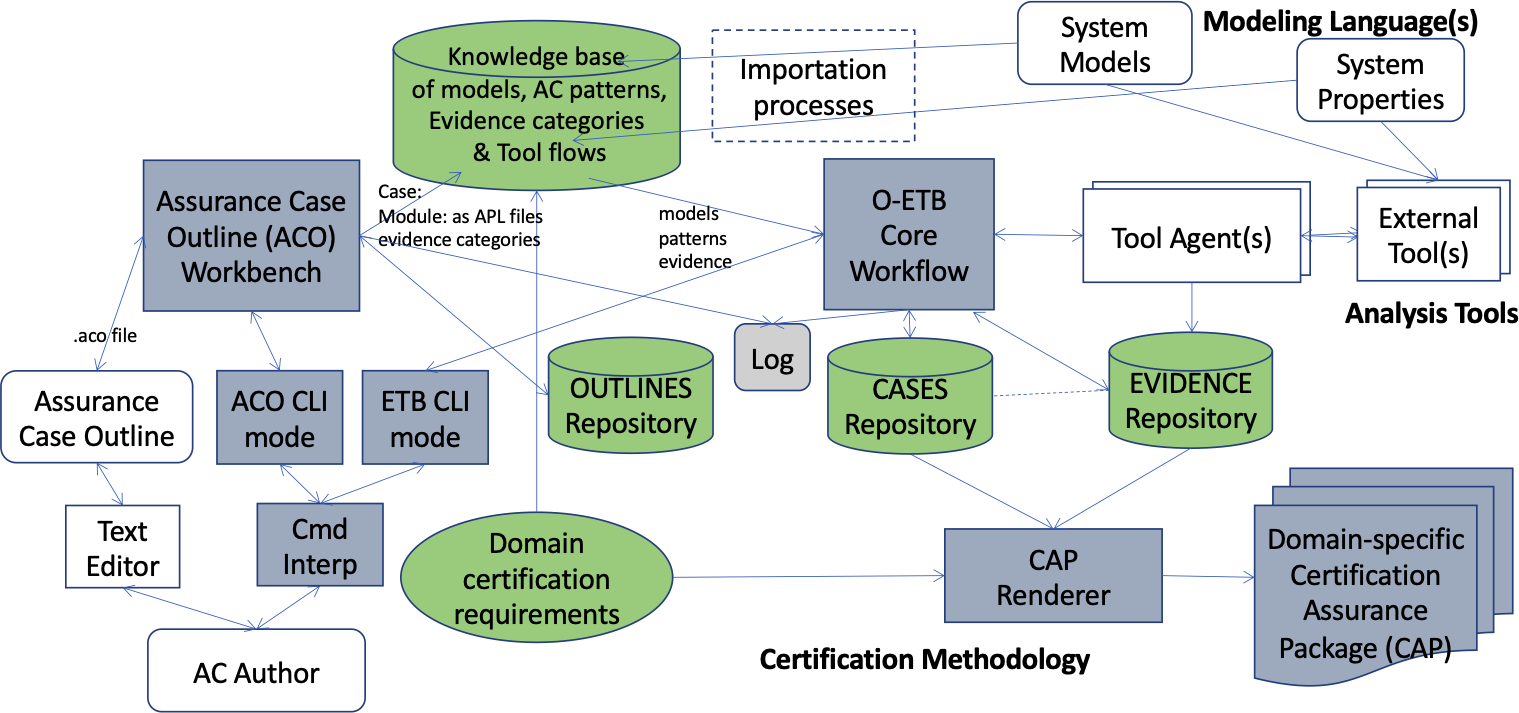
\includegraphics[width=6.5in,height=2.125in]{figures/O-ETB-Final-Arch.pdf}
\caption{O-ETB Functional architecture}\label{fig:etb-arch} 
\end{figure}


\hypertarget{o-etb-components}{%
\subsection{O-ETB components}\label{o-etb-components}}

\hypertarget{functional-components}{%
\subsubsection{Functional components}\label{functional-components}}

\hypertarget{core-workflow-engine}{%
\paragraph{Core Workflow Engine}\label{core-workflow-engine}}

Includes functions that generate instantiated assurance case patterns in the CASES Repository, creates evidence records needed to make the assurance case valid in the EVIDENCE Repository, invokes external evidential tools to validate evidence and to update evidence status in the EVIDENCE repository

\hypertarget{assurance-case-outline-aco-workbench}{%
\paragraph{Assurance Case Outline (ACO) Workbench}\label{assurance-case-outline-aco-workbench}}

The ACO Workbench provides parsing, rendering, analysis, and transformation capabilities for assurance case outlines. It supports tree visualization, statistical analysis, consistency checking, and controlled transformations to internal O-ETB representations.

\hypertarget{interactive-assurance-tool}{%
\paragraph{Interactive Assurance Tool}\label{interactive-assurance-tool}}

The O-ETB has an interactive `etb\textgreater' command mode and an `aco\textgreater' command mode.

\hypertarget{background-assurance-server}{%
\paragraph{Background Assurance Server}\label{background-assurance-server}}

The server is not currently implemented.

\hypertarget{tool-agents}{%
\paragraph{Tool Agent(s)}\label{tool-agents}}

Invocation of executable wrappers for external evidential tools to interface them to O-ETB core workflow and the EVIDENCE Repository.

\hypertarget{cap-renderer}{%
\paragraph{CAP Renderer}\label{cap-renderer}}

Functions to export assurance cases and evidence artefacts in a form to satisfy specific certification evidence presentation requirements.

\hypertarget{kb-import}{%
\paragraph{KB Import}\label{kb-import}}
Though not yet implemented, automated procedures are foreseen for converting external artefacts into KB format artefacts, such as system architectural models and properties of components.

\hypertarget{data-structures-and-storage-components}{%
\subsubsection{Data structures and storage components}\label{data-structures-and-storage-components}}
These constitute mutable but persistent objects that are the intermediate or final results of O-ETB processing that survive executions sessions.


\hypertarget{knowledge-base-1}{%
\paragraph{Knowledge Base}\label{knowledge-base-1}}

Contains several categories of files containing assurance case argument patterns, workflows, system models and properties, evidence category-to-tool mappings, certification artefact requirements, etc.

\hypertarget{assurance-outlines-repository}{%
\paragraph{Assurance OUTLINES Repository}\label{assurance-outlines-repository}}


\hypertarget{assurance-cases-repository}{%
\paragraph{Assurance CASES Repository}\label{assurance-cases-repository}}

Persistent storage of dynamic assurance case elements.

\hypertarget{evidence-repository}{%
\paragraph{EVIDENCE Repository}\label{evidence-repository}}

Persistent storage of evidence records with status and evidential tool results.

%\hypertarget{packaging-of-core-functions}{%
%\subsubsection{Packaging of core functions}\label{packaging-of-core-functions}}

%The O-ETB Assurance Tool and Assurance Server represent two different modes of access to common underlying functionalities of the components identified above, that provide for the construction of assurance cases, including their supporting evidence, and the rendering of these assurance cases with their supporting evidence in a form appropriate for independent evaluation.

%The Assurance Tool provides a command-based interface that can be used interactively and/or in a batch mode to run command scripts. The Assurance Server provides programmatic access to the core functions through an API. Both may be run on a shared centralised file structure, or, for development, testing or experimentation, run on independent instances of the file structure, as determined by configuration options and invocation arguments. As part of that file structure, assurance cases and evidence are constructed incrementally and stored persistently in the CASES and EVIDENCE Repositories respectively.

%Note: The Assurance Server is a work-in-progress and not yet operational for the first prototype.

\hypertarget{certification-assurance-package-1}{%
\paragraph{Certification Assurance Package}\label{certification-assurance-package-1}}

\hypertarget{o-etb-log}{%
\paragraph{O-ETB Log}\label{o-etb-log}}

\hypertarget{component-interactions}{%
\subsection{Component interactions}\label{component-interactions}}

Interaction among O-ETB components is illustrated in the sequence diagram in
Figure~\ref{seq-diag}.



\begin{figure}[htbp]
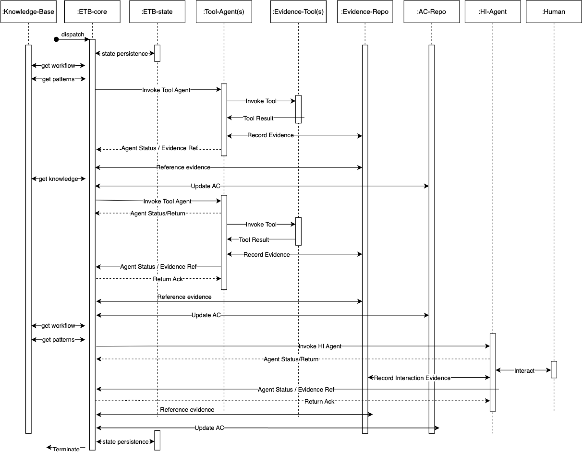
\includegraphics[width=6.125in,height=5.08593in]{figures/image3.png}
\caption{O-ETB component interaction sequence}\label{fig:seq-diag} 
\end{figure}



\protect\hypertarget{_Ref168577340}{}{}Figure 4 Component interaction sequence

Figure~\ref{fig:etb-tool-agents} illustrates the integration of external tools by tool agents.

\begin{figure}[htbp]
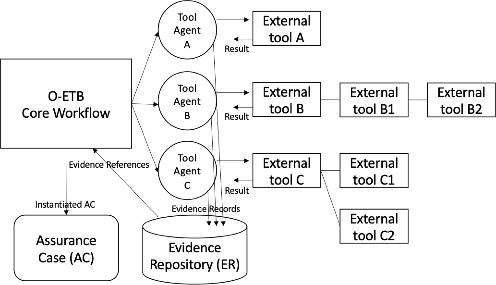
\includegraphics[width=6.5in,height=2.125in]{figures/image4.png}
\caption{O-ETB Tool Agent integration of external tools}\label{fig:etb-tool-agents} 
\end{figure}


\hypertarget{operating-modes}{%
\subsection{Operating modes}\label{operating-modes}}

A summary of the major modes and actions is shown in Figure~\ref{fig:etb-modes}.

\begin{figure}[htbp]
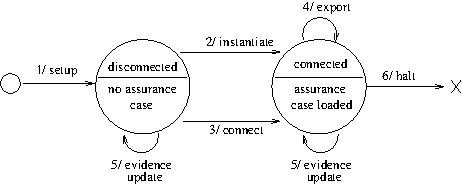
\includegraphics[width=6.125in,height=2.46602in]{figures/image5.png}
\caption{O-ETB major modes and actions}\label{fig:etb-modes} 
\end{figure}


\hypertarget{argument-pattern-instantiation}{%
\subsection{Argument pattern instantiation}\label{argument-pattern-instantiation}}

O-ETB workflow is driven primarily by assurance case argument pattern instantiation. Construction of the argumentation and the generation of the associated supporting evidence is accomplished by the instantiation of a chosen top-level pattern using information from a specified system model.

Figure~\ref{fig:etb-apl-rules} provides the definition of the pattern instantiation rewrite rules.

\begin{figure}[htbp]
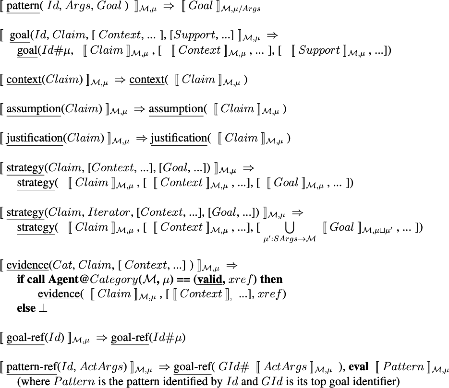
\includegraphics[width=6.5in,height=5.5in]{figures/image6.png}
\caption{Argument pattern grammar and rewrite rules}\label{fig:etb-apl-rules} 
\end{figure}


The following notational conventions are used:
\begin{itemize}
\item
\emph{A} => \emph{C} is a rewrite rule where \emph{A} represents the sentential form to be rewritten and \emph{C} the resultant sentential form.
\item 
\begin{flalign*}[[ Z ]] _{M \mu}\end{flalign*} denotes the instantiation of an assurance case element Z with respect to the model $M$ and using the mapping of formal parameters $\mu$.
\item
  Underlined symbols (e.g. \underline{context}) are terminal symbols of the pattern language.
\item
  Symbols with an initial capital letter (e.g. \emph{Claim}) are logical variables that stand for a term, the type of which is intended to be inferred from the intuitive connotation of the ordinary meaning of the capitalized symbol.
\item
  Bold symbols (e.g. \textbf{eval} or \textbf{if then else}) represent operational semantics.
\item
  An \emph{Iterator} is one of:

  \begin{itemize}
  \item
    \underline{iterate}( \emph{Name}, \emph{Category}, \underline{list}( \emph{Values} ) )
  \item
    \underline{iterate}( \emph{Name}, \emph{Category}, \underline{expand}( \emph{ActArgName} ) )
  \item
    \underline{iterate}( \emph{Name}, \emph{Category}, \underline{subjects}( \emph{PolicyArgName} ) )
  \item
    \underline{iterate}( \emph{Name}, \emph{Category}, \underline{ss\_flows}( \emph{PolicyArgName} ) )
  \item
    \underline{iterate}( \emph{Name}, \emph{Category}, \underline{nodes}( \emph{PolicyArgName} ) )
  \item
    \underline{iterate}( \emph{Name}, \emph{Category}, \underline{modes}( \emph{Subject} ) )
  \item
    \underline{iterate}( \emph{Name}, \emph{Category}, \underline{transitions}( \emph{Subject} ) )
  \end{itemize}
\end{itemize}

\begin{quote}
When the instantiation procedure commences the top-level pattern given to the instantiation procedure becomes the current sentential form to be instantiated. Instantiation proceeds by left-to-right recursive descent on the structure of the form, triggering specific evidence generating tool agents when evidence (leaves) are encountered during pattern instantiation.
\end{quote}

Two cases require a specific treatment beyond the (standard) recursive development:

\begin{itemize}
\item
  The instantiation of an invoked goal (goal-ref) requires the additional instantiation of that goal in the calling context, with the current evaluation of parameters. That is, the instantiation is not limited to the pattern itself but triggers additional instantiation of all other encountered sub-patterns.
\item
  The instantiation of an evidence leaf node requires interaction with the agent associated with the evidence category. When the evidence is valid, it is included in the final result. Otherwise, the assurance case will remain incomplete and the missing evidence is reported to the user.
\end{itemize}

This presentation of the instantiation procedure as a set of rewrite rules has been kept abstract for the sake of exposition. A number of straightforward extensions are however possible, such as the following, that will be considered as the implementation of the O-ETB core workflow evolves:

\begin{itemize}
\item
  memoization of intermediate instantiation results, in particular, to avoid the costly re-generation of the same piece of evidence, referred many times in the assurance cases,
\item
  versioning of segments of the assurance case to work hand-in-hand with memoization to reduce assur- ance case maintenance recompute overhead,
\item
  concurrent execution, that is, allow instantiation to proceed concurrently for independent sub-goals and/or evidence. Such an option might ensure a faster construction process in particular when non-automatic (human-in-the-loop) and/or compute-intensive verification agents are used to produce and check specific evidences,
\item
  additional fine-grained and expressive workflow notation and control mechanisms i.e., choose alternatives based on metrics, depart from depth-first instantiation, exploiting parallelism, restricting or allo- cating execution for some overall time budget, threshold amount of missing evidence, etc.
\end{itemize}

\subsection{Identifier generation and naming during pattern instantiation}
\label{sec:aco-id-generation}

\subsubsection{Unit-scoped identifiers}
In the Assurance Case Outline (ACO) language, outlines are organized into \emph{units}.
A unit is introduced by a \emph{unit header} (for example, \texttt{Case:} or \texttt{Module:}).
Within a unit, the outline consists of \emph{node headers} (for example,
\texttt{Goal}, \texttt{Strategy}, \texttt{Context}, \texttt{Assumption},
\texttt{Justification}, \texttt{Evidence}, and \texttt{Module} nodes).

Identifiers appearing in node headers are \emph{unit-scoped}:
they are required to be unique within the enclosing unit, but they are not required
to be globally unique across different units.
This design supports modular authoring, reuse, and independent development of
assurance case fragments.

\subsubsection{Instantiation and scope lifting}
When a \texttt{Module} unit is instantiated into a concrete assurance case,
all node identifiers defined within that unit must be lifted from unit scope into
a \emph{case-wide} namespace.
This lifting is necessary to ensure that:
\begin{itemize}
  \item multiple modules can be composed within a single assurance case, and
  \item the same module can be instantiated multiple times without identifier collisions.
\end{itemize}

O-ETB performs this lifting during pattern instantiation by allocating a single
\emph{instance identifier} for each \emph{pattern instantiation occurrence}.

\subsubsection{Pattern instantiation occurrence}
A pattern instantiation occurrence corresponds to one concrete expansion of a
\texttt{Module} reference during assurance case construction.
Each occurrence is distinct, even if:
\begin{itemize}
  \item the same module is instantiated multiple times, or
  \item the same module is instantiated multiple times with identical actual arguments.
\end{itemize}

Each occurrence is assigned exactly one instance identifier, which is stable for
the duration of the instantiation and recorded in the assurance case repository
for traceability.

\subsubsection{Construction of instantiated identifiers}
For every node instantiated from a given occurrence, O-ETB derives the
case-wide identifier by concatenating the original unit-scoped identifier
with the instance identifier:
\[
\textit{GlobalId} = \textit{LocalId} \; \texttt{\_} \; \textit{InstanceId}
\]

where:
\begin{itemize}
  \item \textit{LocalId} is the identifier written by the outline author in the
        node header (unit-scoped),
  \item \textit{InstanceId} is the identifier allocated to the instantiation
        occurrence (case-wide), and
  \item \textit{GlobalId} is the identifier that appears in the instantiated
        assurance case and in exported CAP artifacts.
\end{itemize}

For example, if a module defines a goal with identifier \texttt{G10} and that
module is instantiated with instance identifier \texttt{17}, the instantiated
goal identifier becomes \texttt{G10\_17}.

\subsubsection{Properties of the scheme}
This identifier generation scheme ensures that:
\begin{itemize}
  \item identifiers remain readable and retain a clear connection to the
        author-provided outline,
  \item no identifier collisions occur in the instantiated assurance case,
  \item no restrictions are imposed on the syntax of unit-scoped identifiers
        beyond the ACO language definition (including support for canonical
        dotted identifiers), and
  \item all nodes originating from the same pattern instantiation occurrence
        can be recognized by their shared instance identifier.
\end{itemize}

\subsubsection{Relationship to the instantiation workflow}
During assurance case construction, the O-ETB instantiation engine maintains a
set of pending and running pattern instantiations.
Each pending instantiation is represented internally by a triple consisting of:
the referenced module, the bound actual arguments, and the allocated instance
identifier.
All node identifiers produced while instantiating that occurrence are derived
from the same instance identifier, ensuring consistency and traceability across
the instantiated case.

\subsubsection{User-visible effect}
Authors and reviewers will observe the instantiated identifiers (for example,
\texttt{G1\_3}, \texttt{S2\_3}, \texttt{E10\_3}) in generated assurance case
presentations and CAP exports.
These identifiers are tool-generated, deterministic within an instantiation run,
and are intended to provide global uniqueness while preserving a clear relationship
to the original outline structure.


\begin{figure}[htbp]
\centering

\begin{minipage}[t]{0.485\textwidth}
\centering
\textbf{(a) Author outline (unit-scoped IDs)}\\[4pt]

\begin{adjustbox}{max width=\linewidth}
\begin{forest} aco tree
[{\texttt{Case: Main}}
  [{\texttt{Goal G0 Main}}
    [{\texttt{Strategy S0 Decompose}}
      [{\texttt{Goal G1 OpsReadiness}}]
      [{\texttt{Module M1 [secure\_channel(\{Client\},\{Cloud\})]}}
        [{\emph{(module reference; leaf node)}}]
      ]
    ]
  ]
]
\end{forest}
\end{adjustbox}

\vspace{6pt}
{\scriptsize \textit{Referenced module unit (separate unit):}}\\[-2pt]

% Do NOT force this one to full width; cap it (or omit adjustbox entirely).
\begin{adjustbox}{max width=0.85\linewidth}
\begin{forest} aco tree
[{\texttt{Module: secure\_channel(Client,Cloud)}}
  [{\texttt{Goal G10 SecureChannel}}
    [{\texttt{Evidence E10 tlsPolicy}}]
  ]
]
\end{forest}
\end{adjustbox}

\vspace{4pt}
{\scriptsize IDs (e.g., \texttt{G10}, \texttt{E10}) are unique only within their unit.}
\end{minipage}

\vspace{16pt}
\begin{minipage}[t]{0.485\textwidth}
\centering
\textbf{(b) Instantiated case (case-wide IDs)}\\[4pt]

\begin{adjustbox}{max width=\linewidth}
\begin{forest} aco tree
[{\texttt{Case: Main (instantiated)}}
  [{\texttt{Goal G0\_0 Main}}
    [{\texttt{Strategy S0\_0 Decompose}}
      [{\texttt{Goal G1\_0 OpsReadiness}}]
      [{\texttt{Goal G10\_17 SecureChannel}}
        [{\texttt{Evidence E10\_17 tlsPolicy}}]
      ]
    ]
  ]
]
\end{forest}
\end{adjustbox}

\vspace{2pt}
{\scriptsize One instance identifier (\texttt{17}) is allocated for this instantiation occurrence; all nodes from that occurrence share the suffix.}

\end{minipage}

\caption{Example: unit-scoped ACO identifiers lifted to case scope during pattern instantiation}
\label{fig:aco-id-worked-example}
\end{figure}


\hypertarget{knowledge-base-2}{%
\subsection{Knowledge Base}\label{knowledge-base-2}}

\hypertarget{assurance-cases-cases-repository}{%
\subsection{Assurance Cases -- CASES repository}\label{assurance-cases-cases-repository}}

\hypertarget{assurance-case-directories}{%
\subsubsection{Assurance case directories}\label{assurance-case-directories}}

The CASES repository is organised by assurance case identifier.

\hypertarget{persistent-assurance-case-storage}{%
\subsubsection{Persistent assurance case storage}\label{persistent-assurance-case-storage}}

The Assurance Tool and the Assurance Server are designed to build and maintain an assurance case incrementally because there are many distinct assurance activities that contribute to the construction of the assurance case and these activities may be performed over an extended period of time. Intermediate results and even incomplete results must be capable of being captured in one run and to be picked up and used to continue the effort by another run.

O-ETB uses a feature of the Prolog implementation to create, manipulate and store a database of such results and evolving structures. The SWI Prolog library \emph{\textbf{persistency}} provides persistent storage for one or more dynamic predicates. O-ETB employs this feature for several persistent stores, including the CASES Repository and EVIDENCE Repository. O-ETB modules that are responsible for these databases declare the terms that can be placed in the database using the directive \emph{\textbf{persistent}}. By convention and implementation the declaring module is the sole agent having access to the persistent database and provides an internal API to access the database from other modules of the O-ETB system. As there may be multiple instances of the module executing in distinct instances of the Tool or Server, some operations require locking of critical sections in the O-ETB implementation.

\hypertarget{working-assurance-case-cache}{%
\subsubsection{Working assurance case cache}\label{working-assurance-case-cache}}

Each instance of the Assurance Tool or the Assurance Server has a working store for the currently attached assurance case. This cache represents the in-memory copy of the declared persistent predicates and may be synchronized with the persistent CASES Repository, the current assurance case can be detached, and the cache cleared and reloaded with a different assurance case from the Repository.

\hypertarget{assurance-evidence}{%
\subsection{Assurance Evidence}\label{assurance-evidence}}

Evidence is data that provides information about some development artefact (specification, program code, tests, etc) that supports a goal or claim concerning key properties of the artefact that render it fit for purpose. Properties may include security, safety, privacy, functional correctness, performance, etc. Evidence results from performing some assurance activity and capturing the results to be referenced by argumentation for the related goal or claim. Typical assurance activities include:

\begin{itemize}
\item
  Formal verification that system models (which may include formal specifications and/or source code) satisfy formally specified properties or exhibit a required behaviour when executed (actually or symbolically).
\item
  Verifying, by inspection and testing by independent experts, that an artefact or an entire system conforms to applicable and mandated standards.
\item
  Verifying that the specific operating configuration of a system and its deployment and operating environment are consistent with the constraints and assumptions that have been imposed by the development and implementation.
\item
  Analysis of the system architecture, components, and environment to discover potential faults and failures and to determine that appropriate steps have been taken to prevent or to mitigate the effects of such faults and failures. Such analyses may emphasize safety or security or some other characteristic that is essential for the system.
\end{itemize}

\hypertarget{evidence-validation}{%
\subsubsection{Evidence Validation}\label{evidence-validation}}

The assurance processes utilised by MedSecurance involve diverse assurance activities that create concrete evidence artefacts. The collection of evidence artefacts, along with the assurance case that organizes, relates, and presents the evidence, serves as a basis for belief that claims made by the assurance case are valid.

\hypertarget{evidence-artefacts}{%
\subsubsection{Evidence artefacts}\label{evidence-artefacts}}

An evidence artefact is generated by one of multiple potential sources, such as:

\begin{itemize}
\item
  Inspection by a person to confirm a claim such as conformance by a development artefact to an industry standard or a project guideline. Such an inspection action may be entirely manual or may be assisted by one or more tools employed by the inspector that have not been integrated with the automated assurance process.
\item
  A demonstrated and confirmable history of reliable use of a tool for a purpose similar to that for which the tool is being employed to create or support evidence directly used for the present assurance effort.
\item
  Review by qualified experts to confirm that given facts and observations about the entity being assured support a conclusion that is in agreement with a target claim.
\item
  Execution of a test case or collection of test cases in a particular test scenario and configuration to confirm that an expected result is produced.
\item
  Execution of an analysis tool on one or more development artefacts using a specific set of situation-dependent input arguments to confirm that the tool produces an expected result or result that supports a claim.
\end{itemize}

\hypertarget{evidence-categories}{%
\subsubsection{Evidence categories}\label{evidence-categories}}

As discussed previously, for each argument pattern claim or sub-claim requiring substantiation one or more categories of evidence are identified that are capable of supplying the needed substantiation. Each evidence category is associated with a method or tool that is used to produce a concrete evidence artifact of the associated category given the inputs defining the current instance.

The results of performing the method or executing the tool are subject to an interpretation to determine that the result does not represent an exception and that its value is valid and sufficient to support the claim to which it is to be applied.

\hypertarget{evidential-tool-agents}{%
\subsubsection{Evidential tool agents}\label{evidential-tool-agents}}

O-ETB constructs assurance cases that are dependent upon external assurance activities and tools that produce the evidence referenced by the assurance case argumentation. ACs are modular in that they may include assurance goals that are not yet shown to be achieved by the existence of valid evidence. A complete and valid subtree of the AC, for which all needed evidence is complete, can serve as evidence for another goal. Only such reasoning, and tautological reasoning, is performed by the O-ETB itself. For all other evidence, it depends on external processes and tools. Each tool provides a certain class of evidence. When an item of evidence is required to make an element of the AC valid the specified class of the evidence is used to choose a tool agent corresponding to that class.

A tool agent manages the interaction of the O-ETB internal workflow with an external evidence-producing tool. Each tool agent communicates to the core workflow engine through a commonly defined interface and with the evidence repository through its own commonly defined interface. The tool agent embodies the interaction protocol with the specific tool or tool cluster that produces the needed class of evidence. The tool agent marshals the needed arguments, invokes the tool, interprets the tool's response and reports to the core workflow after storing the evidence in the evidence repository. The tool agent is responsible determining success of the evidence validation. That is, the agent must determine that the tool output is consistent with the result needed to satisfy the current goal.

The tool agent is required to perform the following actions:

\begin{itemize}
\item
  marshal the inputs and arguments to the tool in a form the conforms to the requirements of the tool.
\item
  invoke the tool with the collected inputs and arguments.
\item
  monitor the execution and/or receive the results of the tool invocation.
\item
  recognize exceptions raised during the execution of the tool and take appropriate action.
\item
  parse the results and interpret them to the extent necessary to determine that they conform to the expected format, that they do not represent an error condition, and that they appear to represent a valid outcome. The validation status is recorded appropriately as `valid' or `invalid'.
\item
  store the outcome in an evidence record of the EVIDENCE Repository in a canonical form that has been defined for the corresponding evidence category, and the status is recorded.
\item
  depending on whether the tool agent was launched for synchronous, asynchronous or silent operation return to the O-ETB core workflow, signal completion to the O-ETB server through its API, or silently exit.
\item
  when the validation status of a tool invocation or manual assurance activity cannot definitively be reported as `valid' or `invalid' by the tool agent it is reported as `ongoing'.
\end{itemize}

For evidence checking that reports a validation status of `ongoing' the validation activity continues asynchronously with respect to O-ETB (for example as a manual process carried out by people). In such cases, once a definitive verdict of `valid' or `invalid' is reached the validation status file is updated either by the asynchronously running tool agent or by the Server's workflow program upon notification through the API.

In some cases, a group of external tools work in concert under the coordination of, and invoked by, a control process. In such cases the tool agent is designed to interface only with the control process and to leave the sequencing and communication with and among the other tools to the control process.

Evidence categories that correspond to assurance activities performed manually by one or more people, whether or not the activity is supported by tools outside of the O-ETB workflow, are included in the O-ETB workflow through special UI agents that deliver the relevant facts to a designated responsible individual who will in turn respond to the UI agent or programmatically invoke the Server API to report results of the assigned activity.

\hypertarget{evidence-artefact-validation-status}{%
\subsubsection{Evidence artefact validation status}\label{evidence-artefact-validation-status}}

The previous paragraph alludes to the validation status of an evidence artefact. The validation status is contained within a status file that is created within the EVIDENCE Repository when the artefact is initially created. Upon creation the status is recorded as `pending'.

\hypertarget{re-synchronisation}{%
\subsubsection{Re-synchronisation}\label{re-synchronisation}}

EVIDENCE Repository updates by asynchronous tool agents do not immediately result in update to assurance cases that are supported by the evidence artefacts. Rather, update of assurance cases occurs when manually initiated by the user of the Assurance Tool or by the Assurance Server either periodically or when prompted through an API request.

\hypertarget{evidence-repository-1}{%
\subsection{EVIDENCE repository}\label{evidence-repository-1}}

\hypertarget{evidence-category-directories}{%
\subsubsection{Evidence category directories}\label{evidence-category-directories}}

Evidence records of a particular evidence category are stored in a subdirectory named for the category.

\hypertarget{persistent-evidence-storage}{%
\subsubsection{Persistent evidence storage}\label{persistent-evidence-storage}}

A Prolog feature for persistent data bases is used for the evidence storage. The Prolog program manipulates a copy of the data in memory which is automatically synced to a file in the file system for persistence.

\hypertarget{working-evidence-cache}{%
\subsubsection{Working evidence cache}\label{working-evidence-cache}}

The running Assurance Tool or Assurance Server maintains a local working cache of evidence records that are backed by the persistent EVIDENCE Repository.

\hypertarget{outlines-repository}{%
\subsection{OUTLINES repository}\label{outlines-repository}}

\protect\hypertarget{_Toc217342243}{}{}The OUTLINES Repository is the persistent store for assurance case outlines and their derived internal forms. It supports continuity across sessions and enables traceability from outline evolution to instantiated cases and published CAP artifacts.\\
\strut \\
In addition to source ACO files, the repository may store parsed/canonical internal representations, transformation results, and metadata (including provenance and tool versions), together with any Workbench state required to reproduce assessments, diagnostics, and views. OUTLINES is distinct from CASES (instantiated cases) and EVIDENCE (supporting artifacts), reflecting the lifecycle separation between outline development, instantiation, and evidence management (MedSecurance Project, 2025a).

\hypertarget{certification-assurance-package-cap}{%
\subsection{Certification Assurance Package (CAP)}\label{certification-assurance-package-cap}}

The certification assurance package is a collection of artefacts, rendered from data in the CASES and EVIDENCE Repositories, into a form that is suitable for presentation as part of an application for certification under a particular certification regime.

\hypertarget{tailoring-the-cap-to-certification-requirements}{%
\subsubsection{Tailoring the CAP to certification requirements}\label{tailoring-the-cap-to-certification-requirements}}

Figure~\ref{fig:cert-rqmts} illustrates how domain-specific certification regime requirements can be used to control the evidence generation processes, the operation of the ETB, the structure of the assurance case and the final rendered content of the CAP for a specific certification regime or project.

\begin{figure}[htbp]
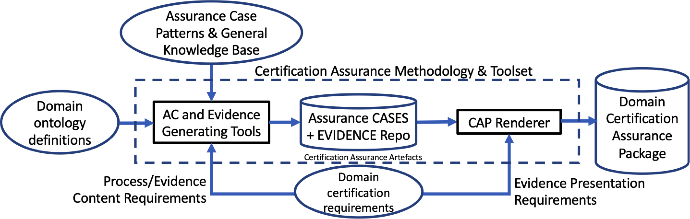
\includegraphics[width=6.125in,height=2.08593in]{figures/image7.png}
\caption{Tailoring the CAP to certification requirements}\label{fig:cert-rqmts} 
\end{figure}

\hypertarget{organising-multiple-certification-projects}{%
\subsubsection{Organising multiple certification projects}\label{organising-multiple-certification-projects}}

Currently the staging area for certification assurance artefacts is a single directory named ``CAP''. Since the export operations of the O-ETB enable the file and directory names for the exported items to be specified, a user-chosen naming convention can assist in managing the contents of the CAP directory. Notwithstanding this possibility it would be useful to provide organisation within the CAP directory as a standard feature of O-ETB and this is anticipated as a future extension. This extension would include commands and APIs that provide the ability to register a certification project. The certification registry could be maintained as persistent database at the top-level of the CAP directory. Then, using the certification project identifier as a key, the maintenance of the process and presentation requirements of the certification could be stored in the Knowledge Base and the suitably presented artefacts could be organized in the CAP by subdirectories named for the project identifiers.

\hypertarget{text-file-artefacts}{%
\subsubsection{Text file artefacts}\label{text-file-artefacts}}

Assurance cases can be exported in textual form in a .txt file of specified name.

\hypertarget{html-directory-artefacts}{%
\subsubsection{HTML directory artefacts}\label{html-directory-artefacts}}

Assurance cases can be exported in graphical form as a collection of HTML files in a specified directory name. An ordinary web browser may be used to navigate the AC.

\clearpage
\hypertarget{assurance-tool-examples}{%
\section{Assurance Tool Examples}\label{assurance-tool-examples}}

Several examples of the use of the Assurance Tool have been encoded as procs in the file procs.pl. To gain familiarity with interactive use of the tool the commands defining these procs may be entered interactively one-at-a-time. When this is done each command must terminate with a ``.''.

No Assurance Server examples are presented. Further implementation of the Assurance Server has been deferred unless a clear need for it arises in the MedSecurance Project. The current workflow of the MedSecurance methodology involves interactive and scripted operation of the Assurance tools and does not require programmatic invocation of the O-ETB functions. All automatically sequenced use of the functions can be currently be adequately accomplished by predefined command procs and scripts.

\hypertarget{example-1-o-etb-tool-instantiating-a-simple-pattern}{%
\subsection{Example 1 -- O-ETB Tool instantiating a simple pattern}\label{example-1-o-etb-tool-instantiating-a-simple-pattern}}

This example is encoded as the person\_inst procedure in procs\_etb.pl as shown in Table 4.

\begin{longtable}[]{@{}
  >{\raggedright\arraybackslash}p{(\columnwidth - 0\tabcolsep) * \real{1.0000}}@{}}
\caption{\protect\hypertarget{_Ref168411618}{}{}Table Example 1 -- instantiating a simple pattern and exporting the result}\tabularnewline
\toprule
\begin{minipage}[b]{\linewidth}\raggedright
proc(person\_inst, {[}\\
instantiate\_pattern(person, {[}'Marius', 'Programming'{]}, person\_examp),\\
ac\_export(cap\_person,txt),\\
detach\_case\\
{]}).\strut
\end{minipage} \\
\midrule
\endfirsthead
\toprule
\begin{minipage}[b]{\linewidth}\raggedright
proc(person\_inst, {[}\\
instantiate\_pattern(person, {[}'Marius', 'Programming'{]}, person\_examp),\\
ac\_export(cap\_person,txt),\\
detach\_case\\
{]}).\strut
\end{minipage} \\
\midrule
\endhead
\bottomrule
\end{longtable}

In this procedure the command instantiate\_pattern causes the pattern person to be instantiated with the arguments given in the list and will be stored in the CASES Repository with the case identifier person\_examp.

Table 5 shows a transcript of listing and executing the person\_inst procedure with the optional verbose argument. It instantiates the pattern ``person'' and creates the assurance case ``person\_examp'' in the CASES Repository.

\begin{longtable}[]{@{}
  >{\raggedright\arraybackslash}p{(\columnwidth - 0\tabcolsep) * \real{1.0000}}@{}}
\caption{\protect\hypertarget{_Ref175577865}{}{}Table 5 Running the person\_inst procedure}\tabularnewline
\toprule
\begin{minipage}[b]{\linewidth}\raggedright
etb\textgreater{} show\_proc(person\_inst).

:- dynamic procs:proc/2.

procs:proc(person\_inst,

{[} instantiate\_pattern(person, {[}'Marius', 'Programming'{]}, person\_examp),

export\_case(cap\_person, txt),

detach\_case

{]}).

etb\textgreater{} proc(person\_inst,verbose).

\textgreater{} instantiate\_pattern(person,{[}'Marius','Programming'{]},person\_examp).

*** instantiating pattern person ... done.

goal g0\_1 : \{Marius\} is sufficiently trustworthy

goal g1\_2 : \{Marius\} has the necessary attributes to perform \{Programming\}

strategy : argument over attributes

goal g11\_3 : \{Marius\} has sufficient \{capability\} to perform \{Programming\}

evidence certificate : \{Marius\} \{capability\} for \{Programming\}

ongoing reference -\textgreater{} 10001

goal g11\_4 : \{Marius\} has sufficient \{experience\} to perform \{Programming\}

evidence certificate : \{Marius\} \{experience\} for \{Programming\}

ongoing reference -\textgreater{} 10002

goal g2\_5 : \{Marius\} has sufficient level of supervision and review to successfully perform \{Programming\}

\textgreater{} export\_case(cap\_person,txt).

\textgreater{} detach\_case.

etb\textgreater{}
\end{minipage} \\
\midrule
\endfirsthead
\toprule
\begin{minipage}[b]{\linewidth}\raggedright
etb\textgreater{} show\_proc(person\_inst).

:- dynamic procs:proc/2.

procs:proc(person\_inst,

{[} instantiate\_pattern(person, {[}'Marius', 'Programming'{]}, person\_examp),

export\_case(cap\_person, txt),

detach\_case

{]}).

etb\textgreater{} proc(person\_inst,verbose).

\textgreater{} instantiate\_pattern(person,{[}'Marius','Programming'{]},person\_examp).

*** instantiating pattern person ... done.

goal g0\_1 : \{Marius\} is sufficiently trustworthy

goal g1\_2 : \{Marius\} has the necessary attributes to perform \{Programming\}

strategy : argument over attributes

goal g11\_3 : \{Marius\} has sufficient \{capability\} to perform \{Programming\}

evidence certificate : \{Marius\} \{capability\} for \{Programming\}

ongoing reference -\textgreater{} 10001

goal g11\_4 : \{Marius\} has sufficient \{experience\} to perform \{Programming\}

evidence certificate : \{Marius\} \{experience\} for \{Programming\}

ongoing reference -\textgreater{} 10002

goal g2\_5 : \{Marius\} has sufficient level of supervision and review to successfully perform \{Programming\}

\textgreater{} export\_case(cap\_person,txt).

\textgreater{} detach\_case.

etb\textgreater{}
\end{minipage} \\
\midrule
\endhead
\bottomrule
\end{longtable}

As part of the verbose setting the text of the resulting instantiated assurance case pattern is also sent to the console in text form. It is important to execute the command ``detach\_case'' after working with a new AC.

In the procedure of this example the command export\_case causes the assurance case in the working cache to be exported to the CAP directory as text in the file cap\_person.txt, which you can inspect for yourself.

\hypertarget{example-2-assurance-tool-exporting-an-assurance-case}{%
\subsection{Example 2 -- Assurance Tool exporting an assurance case}\label{example-2-assurance-tool-exporting-an-assurance-case}}

The next example is the procedure ``person\_exp'' (for person export) in Table 6 shows operations on the already existing instantiated pattern stored in the CASES Repository under the identifier ``person\_examp''.

This example is encoded as the person\_exp procedure in procs\_etb.pl as shown in Table 6.

\begin{longtable}[]{@{}
  >{\raggedright\arraybackslash}p{(\columnwidth - 0\tabcolsep) * \real{1.0000}}@{}}
\caption{\protect\hypertarget{_Ref168411722}{}{}Table Example 2 -- exporting an assurance case as HTML}\tabularnewline
\toprule
\begin{minipage}[b]{\linewidth}\raggedright
proc(person\_exp, {[}\\
update,\\
attach\_case(person\_examp),\\
ac\_export(cap\_person,html),\\
detach\_case\\
{]}).\strut
\end{minipage} \\
\midrule
\endfirsthead
\toprule
\begin{minipage}[b]{\linewidth}\raggedright
proc(person\_exp, {[}\\
update,\\
attach\_case(person\_examp),\\
ac\_export(cap\_person,html),\\
detach\_case\\
{]}).\strut
\end{minipage} \\
\midrule
\endhead
\bottomrule
\end{longtable}

Table 7 shows a transcript that lists and executes the person\_exp procedure with the optional verbose argument.

\begin{longtable}[]{@{}
  >{\raggedright\arraybackslash}p{(\columnwidth - 0\tabcolsep) * \real{1.0000}}@{}}
\caption{\protect\hypertarget{_Ref175579287}{}{}Table 7 Running the person\_exp procedure}\tabularnewline
\toprule
\begin{minipage}[b]{\linewidth}\raggedright
etb\textgreater{} show\_proc(person\_exp).

:- dynamic procs:proc/2.

procs:proc(person\_exp,

{[} update,

attach\_case(person\_examp),

export\_case(cap\_person, html),

detach\_case

{]}).

etb\textgreater{} proc(person\_exp,verbose).

\textgreater{} update.

*** updating evidence repository ... done.

\textgreater{} attach\_case(person\_examp).

\textgreater{} export\_case(cap\_person,html).

\textgreater{} detach\_case.

etb\textgreater{}
\end{minipage} \\
\midrule
\endfirsthead
\toprule
\begin{minipage}[b]{\linewidth}\raggedright
etb\textgreater{} show\_proc(person\_exp).

:- dynamic procs:proc/2.

procs:proc(person\_exp,

{[} update,

attach\_case(person\_examp),

export\_case(cap\_person, html),

detach\_case

{]}).

etb\textgreater{} proc(person\_exp,verbose).

\textgreater{} update.

*** updating evidence repository ... done.

\textgreater{} attach\_case(person\_examp).

\textgreater{} export\_case(cap\_person,html).

\textgreater{} detach\_case.

etb\textgreater{}
\end{minipage} \\
\midrule
\endhead
\bottomrule
\end{longtable}

The procedure first performs a precautionary call to the update command, which will cause any pending updates to the repositories to be synchronized.

After performing any pending updates the procedure attaches the previously existing case (``person\_examp'') and then exports it as a directory named CAP/cap\_person containing the HTML representation components.

An ordinary browser can be used to open the CAP/cap\_person/index.html file in the new directory. By clicking on the different elements listed on the left (in this simple example there is only one element ``person\_g0\_1'') you can see the graphical representation as shown in Figure~\ref{fig:pers-pat} shows the instantiation of the person pattern.

\begin{figure}[htbp]
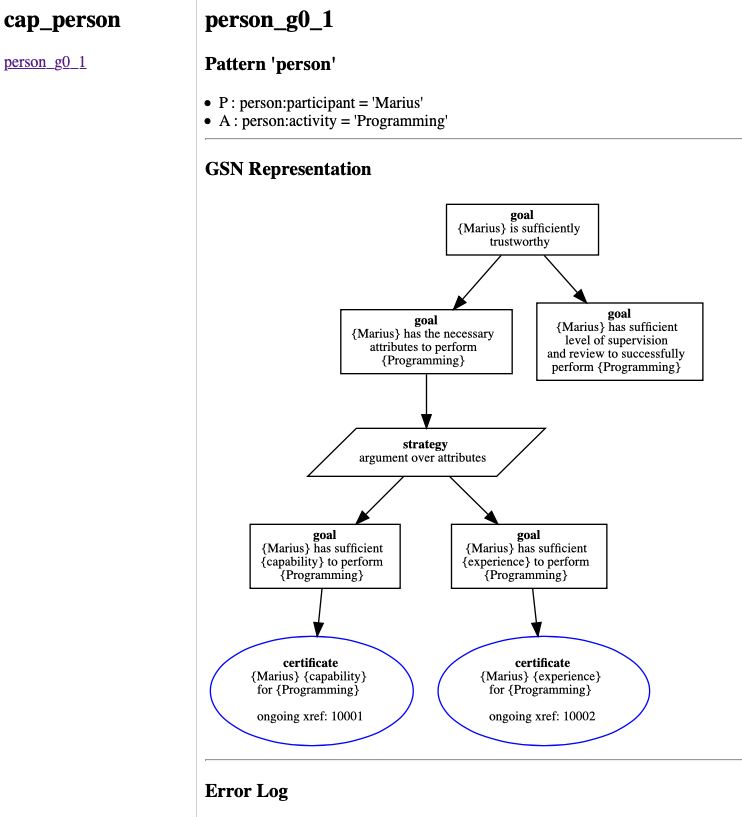
\includegraphics[width=6.125in,height=6.5in]{figures/image8.png}
\caption{Argument pattern instantiation for a person}\label{fig:pers-pat} 
\end{figure}


\hypertarget{example-3-assurance-tool-loading-a-model-and-instantiating-a-pattern-list}{%
\subsection{Example 3 -- Assurance Tool loading a model and instantiating a pattern list}\label{example-3-assurance-tool-loading-a-model-and-instantiating-a-pattern-list}}

This example is encoded as the system\_inst procedure in procs\_etb.pl as shown in Table 8.

\begin{longtable}[]{@{}
  >{\raggedright\arraybackslash}p{(\columnwidth - 0\tabcolsep) * \real{1.0000}}@{}}
\caption{\protect\hypertarget{_Ref168412244}{}{}Table Example 3 -- instantiating a pattern list from a model and exporting as HTML}\tabularnewline
\toprule
\begin{minipage}[b]{\linewidth}\raggedright
proc(system\_inst, {[}\\
set\_v(ModelId, `1.0'),\\
set\_v(CaseId, system\_examp),\\
load\_model\_v(ModelId, Policy, Platform, \_Configuration),\\
set\_v(AC, {[}\\
`foundational\_plane'-{[}Platform{]},\\
`operational\_plane'-{[}Policy{]},\\
`person'-{[}`Alice', `AC Patterns Definition'{]},\\
`person'-{[}`Bob', `ETB Development{]}\\
{]}),\\
instantiate\_pattern\_list(AC, CaseId),\\
ac\_export(CaseId, html),\\
detach\_case\\
{]}).\strut
\end{minipage} \\
\midrule
\endfirsthead
\toprule
\begin{minipage}[b]{\linewidth}\raggedright
proc(system\_inst, {[}\\
set\_v(ModelId, `1.0'),\\
set\_v(CaseId, system\_examp),\\
load\_model\_v(ModelId, Policy, Platform, \_Configuration),\\
set\_v(AC, {[}\\
`foundational\_plane'-{[}Platform{]},\\
`operational\_plane'-{[}Policy{]},\\
`person'-{[}`Alice', `AC Patterns Definition'{]},\\
`person'-{[}`Bob', `ETB Development{]}\\
{]}),\\
instantiate\_pattern\_list(AC, CaseId),\\
ac\_export(CaseId, html),\\
detach\_case\\
{]}).\strut
\end{minipage} \\
\midrule
\endhead
\bottomrule
\end{longtable}

This procedure uses the logical variables ModelId, CaseId, Policy, Platform, \_Configuration and AC to represent values in the procedure (see Section 2.2.3 for notes on syntactic conventions). The transcript of the execution of this procedure is rather lengthy with the verbose option and is not reproduced here. However, it is instructive to use a browser to view the exported HTML in CAP/system\_examp directory as this represents a more extensive example.

%\hypertarget{example-4-medsecurance-rpms-example-wip}{%
%\subsection{Example 4 -- MedSecurance RPMS example (WIP)}\label{example-4-medsecurance-rpms-example-wip}}

%This example is a commentary on approaches to the use of O-ETB within the Remote Patient Monitoring System example given in MedSecurance D3.1. It is a work in progress.

%There are several possible usage scenarios, depending on the IoMT system developer's workflow, availability and choice of tools, the extent of the implementation of O-ETB features at the time, the extent of experience gained in using MedSecurance methodology, the extend of experience gained with MedSecurance analysis tools, and the encoding of that experience as assurance case patterns and tool application patterns.

%\begin{itemize}
%\item
%  Scenario 1 -- manual encoding of O-ETB model data from models developed with modelling tools
%\item
%  Scenario 2 -- (semi-)automatic encoding of O-ETB model data from models
%\item
%  Scenario 3 -- no pre-existing and complete assurance case pattern for a particular target certification
%\item
%  Scenario 4 -
%\end{itemize}

%Other factors that will affect the approach:

%\begin{enumerate}
%\def\labelenumi{\arabic{enumi}.}
%\item
%  Existence of one or more general architectural models applicable to the particular RPMS example
%\item
%  Existence of automated extraction/translation of O-ETB model and property information from MedSecurance modelling tool outputs.
%\item
%  Existence of completed assurance case patterns embodying the MedSecurance methodology and targeting a particular target certification.
%\item
%  Existence of tool agents to automate all tool runs.
%\item
%  Availability of sufficiently mature versions of all modelling and analysis tools.
%\end{enumerate}

\begin{longtable}[]{@{}
  >{\raggedright\arraybackslash}p{(\columnwidth - 8\tabcolsep) * \real{0.2001}}
  >{\raggedright\arraybackslash}p{(\columnwidth - 8\tabcolsep) * \real{0.1999}}
  >{\raggedright\arraybackslash}p{(\columnwidth - 8\tabcolsep) * \real{0.1999}}
  >{\raggedright\arraybackslash}p{(\columnwidth - 8\tabcolsep) * \real{0.1999}}
  >{\raggedright\arraybackslash}p{(\columnwidth - 8\tabcolsep) * \real{0.2001}}@{}}
\caption{\protect\hypertarget{_Ref192627937}{}{}Table Abbreviations}\tabularnewline
\toprule
\begin{minipage}[b]{\linewidth}\raggedright
\end{minipage} & \begin{minipage}[b]{\linewidth}\raggedright
\end{minipage} & \begin{minipage}[b]{\linewidth}\raggedright
\end{minipage} & \begin{minipage}[b]{\linewidth}\raggedright
\end{minipage} & \begin{minipage}[b]{\linewidth}\raggedright
\end{minipage} \\
\midrule
\endfirsthead
\toprule
\begin{minipage}[b]{\linewidth}\raggedright
\end{minipage} & \begin{minipage}[b]{\linewidth}\raggedright
\end{minipage} & \begin{minipage}[b]{\linewidth}\raggedright
\end{minipage} & \begin{minipage}[b]{\linewidth}\raggedright
\end{minipage} & \begin{minipage}[b]{\linewidth}\raggedright
\end{minipage} \\
\midrule
\endhead
& & & & \\
& & & & \\
& & & & \\
& & & & \\
\bottomrule
\end{longtable}

\clearpage
\hypertarget{references}{%
\section{References}\label{references}}

\begin{enumerate}
\def\labelenumi{\arabic{enumi}.}
\item
  Medical Device Coordination Group (MDCG), https://ec.europa.eu/transparency/expert-groups-register/screen/expert-groups/consult?lang=en\&groupID=3565
\item
  Interfaces and Workflow Definition for AM-ETB, CITADEL Project D5.1, May 2017.
\item
  AM-ETB Tool Bus for Tool Integration and Assurance, CITADEL Project D5.2, May 2018.
\item
  CITADEL project, http://www.citadel-project.org, 2019.
\item
  ISO/TC 215 CD 81001-2-1 Assurance cases, draft for comment, 18 December 2023.
\item
  N. Shankar, et al, DesCert: Design for Certification, SRI International, arXiv:2203.15178, March 2022.
\item
  Goal Structuring Notation Community Standard Version 3, The Assurance Case Working Group (ACWG), SCSC-141C, May 2021.
\item
  Y. Matsuno, Design and Implementation of GSN Patterns: A Step toward Assurance Case Language, In-formation Processing Society of Japan, IPSJ Transactions on Programming 7(2):1-10, 2014.
\item
  S. Gregory and M. Paschali, A Prolog-based language for workflow programming, University of Bristol, technical report CSTR-07-001, February 2007; and Proceedings of the 9th International Conference on Coordination Models and Languages, June 2007.
\item
  Object Management Group (OMG), Structured Assurance Case Metamodel (SACM), Version 2.0, 2018.
\item
  Medical Device Coordination Group, ``MDCG 2019-11~Guidance on Qualification and Classification of Software in Regulation (EU) 2017/745 -- MDR~and Regulation (EU) 2017/746 -- IVDR'' Oct. 2019.
\item
  Medical Device Coordination Group, ``MDCG 2019-16 Rev.1 Guidance on Cybersecurity for medical devices,'' 2020.
\item
  MedSec-Sec Control Taxonomy v2, \href{https://github.com/MedSecurance/Internal/tree/main/WPs/WP3/OntologyWork/MedSec-Sec_Control_Taxonomy_Version\%200.2.xlsx}{https://github.com/MedSecurance/Internal/tree/main/WPs/WP3/OntologyWork/MedSec-Sec\_Control\_Taxonomy\_Version 0.2.xlsx} .
\item
  J. Rushby, An Evidential Tool Bus. In Formal Methods and Software Engineering, 7\textsuperscript{th} International Conference on Formal Engineering Methods (ICFEM), 2005.
\item
  N. Selviandro, Assurance case pattern using SACM notation. In 2021 9\textsuperscript{th} International Conference on Information and Communication Technology (ICoICT), pp. 494-499. IEEE, 2021.
\item
  R. Wei, T. P. Kelly, X. Dai, S. Zhao, and R. Hawkins, Model based system assurance using the structured assurance case metamodel. Journal of Systems and Software, 154:211-233, 2019.
\item
  T. A. Beyene and Harald Ruess, Evidential and Continuous Integration of Software Verification Tools. Proceedings 22\textsuperscript{nd} International Symposium, FM, FLoC, 2018.
\end{enumerate}

\clearpage
\hypertarget{abbreviations}{%
\section{Abbreviations}\label{abbreviations}}

Table 9 lists the meanings of acronyms and abbreviations used in this User Manual. A comprehensive collection of abbreviations and terms used in the broader context of the use of O-ETB is referenced in Annex E: Assurance Glossary.

\begin{longtable}[]{@{}
  >{\raggedright\arraybackslash}p{(\columnwidth - 2\tabcolsep) * \real{0.2701}}
  >{\raggedright\arraybackslash}p{(\columnwidth - 2\tabcolsep) * \real{0.7299}}@{}}
\caption{\protect\hypertarget{_Ref160560465}{}{}Table 10 O-ETB v1.1.3 directory tree}\tabularnewline
\toprule
\begin{minipage}[b]{\linewidth}\raggedright
AC
\end{minipage} & \begin{minipage}[b]{\linewidth}\raggedright
Assurance Case
\end{minipage} \\
\midrule
\endfirsthead
\toprule
\begin{minipage}[b]{\linewidth}\raggedright
AC
\end{minipage} & \begin{minipage}[b]{\linewidth}\raggedright
Assurance Case
\end{minipage} \\
\midrule
\endhead
A-G & Assume-Guarantee \\
CR & CASES Repository \\
CAP & Certification Assurance Package \\
CWE & Core Workflow Engine \\
ER & EVIDENCE Repository \\
ETB & Evidential Tool Bus \\
GSN & Goal Structuring Notation \\
KB & Knowledge Base (O-ETB component) \\
LTL & Linear Temporal Logic \\
MS & MedSecurance \\
O-ETB & Open ETB \\
OMG & Object Management Group \\
SACM & Structured Assurance Case Metamodel -- a standard from OMG for expressing assurance cases and evidence \\
TA & Tool Agent components \\
\bottomrule
\end{longtable}

\clearpage
\hypertarget{annex-a-o-etb-configuration-identification}{%
\section{Annex A: O-ETB Configuration Identification}\label{annex-a-o-etb-configuration-identification}}

\hypertarget{file-identification}{%
\subsection{File identification}\label{file-identification}}

The directory tree of the O-ETB v1.1.3 source repository and distribution is given in Table 8. A description of the contents and purposes of these directories and files is covered in Section 2.1 and a description of the contents of the files containing source code modules in Section 8.2.

\begin{longtable}[]{@{}
  >{\raggedright\arraybackslash}p{(\columnwidth - 2\tabcolsep) * \real{0.5378}}
  >{\raggedright\arraybackslash}p{(\columnwidth - 2\tabcolsep) * \real{0.4622}}@{}}
\caption{\protect\hypertarget{_Ref160560217}{}{}Table 11 O-ETB v1.1.3 source code modules}\tabularnewline
\toprule
\begin{minipage}[b]{\linewidth}\raggedright
./REPOSITORY/EVIDENCE

./REPOSITORY/EVIDENCE/certificate

./REPOSITORY/EVIDENCE/certificate/README.md

./REPOSITORY/EVIDENCE/axiom

./REPOSITORY/EVIDENCE/axiom/README.md

./REPOSITORY/EVIDENCE/README.md

./REPOSITORY/EVIDENCE/ocra

./REPOSITORY/EVIDENCE/ocra/README.md

./REPOSITORY/EVIDENCE/unknown

./REPOSITORY/EVIDENCE/unknown/README.md

./REPOSITORY/EVIDENCE/repository.pl

./REPOSITORY/EVIDENCE/ichecker

./REPOSITORY/EVIDENCE/ichecker/README.md

./REPOSITORY/CASES

./REPOSITORY/CASES/README.md

./REPOSITORY/README.md

./LICENSE

./KB/PATTERNS

./KB/PATTERNS/patterns\_ISO\_81001.pl

./KB/PATTERNS/patterns\_MILS.pl

./KB/MODELS/1.0

./KB/MODELS/1.0/configuration.pl

./KB/MODELS/1.0/system-invariants.inv

./KB/MODELS/1.0/policy.pl

./KB/MODELS/1.0/platform.pl

./KB/MODELS/1.0/properties

./KB/MODELS/1.0/properties/p1.pro

./KB/MODELS/1.0/properties/p2.pro

./KB/MODELS/1.0/system.bip

./KB/README.md\\
./KB/WORKFLOWS

./docs/README-O-ETB-v1

./docs/README-AM-ETB-v3

./docs/O-ETB-v1.1.0-User-Manual.pdf

./README.md

./CAP/README.md

./BUILD/etb\\
./BUILD/README.md\\
./TEST/README.md\strut
\end{minipage} & \begin{minipage}[b]{\linewidth}\raggedright
./src/stringutil.pl

./src/models\_api/configuration.pl

./src/models\_api/policy.pl

./src/models\_api/model.pl

./src/models\_api/platform.pl

./src/models\_api/common.pl

./src/patterns.pl

./src/procs\_etb.pl

./src/makefile

./src/etb\_server.pl

./src/etb.pl

./src/agents/ocra\_agent.pl

./src/agents/axiom\_agent.pl

./src/agents/ichecker\_agent.pl

./src/agents/certificate\_agent.pl

./src/export.pl

./src/assurance.pl

./src/instantiate.pl

./src/agent.pl

./src/command\_etb.pl

./src/demo.pl\\
./src/kb.pl

./src/com/command.pl

./src/com/ui.pl

./src/com/param.pl

./src/com/test.pl

./src/com/README.md

./src/com/procs.pl

./src/evidence.pl\strut
\end{minipage} \\
\midrule
\endfirsthead
\toprule
\begin{minipage}[b]{\linewidth}\raggedright
./REPOSITORY/EVIDENCE

./REPOSITORY/EVIDENCE/certificate

./REPOSITORY/EVIDENCE/certificate/README.md

./REPOSITORY/EVIDENCE/axiom

./REPOSITORY/EVIDENCE/axiom/README.md

./REPOSITORY/EVIDENCE/README.md

./REPOSITORY/EVIDENCE/ocra

./REPOSITORY/EVIDENCE/ocra/README.md

./REPOSITORY/EVIDENCE/unknown

./REPOSITORY/EVIDENCE/unknown/README.md

./REPOSITORY/EVIDENCE/repository.pl

./REPOSITORY/EVIDENCE/ichecker

./REPOSITORY/EVIDENCE/ichecker/README.md

./REPOSITORY/CASES

./REPOSITORY/CASES/README.md

./REPOSITORY/README.md

./LICENSE

./KB/PATTERNS

./KB/PATTERNS/patterns\_ISO\_81001.pl

./KB/PATTERNS/patterns\_MILS.pl

./KB/MODELS/1.0

./KB/MODELS/1.0/configuration.pl

./KB/MODELS/1.0/system-invariants.inv

./KB/MODELS/1.0/policy.pl

./KB/MODELS/1.0/platform.pl

./KB/MODELS/1.0/properties

./KB/MODELS/1.0/properties/p1.pro

./KB/MODELS/1.0/properties/p2.pro

./KB/MODELS/1.0/system.bip

./KB/README.md\\
./KB/WORKFLOWS

./docs/README-O-ETB-v1

./docs/README-AM-ETB-v3

./docs/O-ETB-v1.1.0-User-Manual.pdf

./README.md

./CAP/README.md

./BUILD/etb\\
./BUILD/README.md\\
./TEST/README.md\strut
\end{minipage} & \begin{minipage}[b]{\linewidth}\raggedright
./src/stringutil.pl

./src/models\_api/configuration.pl

./src/models\_api/policy.pl

./src/models\_api/model.pl

./src/models\_api/platform.pl

./src/models\_api/common.pl

./src/patterns.pl

./src/procs\_etb.pl

./src/makefile

./src/etb\_server.pl

./src/etb.pl

./src/agents/ocra\_agent.pl

./src/agents/axiom\_agent.pl

./src/agents/ichecker\_agent.pl

./src/agents/certificate\_agent.pl

./src/export.pl

./src/assurance.pl

./src/instantiate.pl

./src/agent.pl

./src/command\_etb.pl

./src/demo.pl\\
./src/kb.pl

./src/com/command.pl

./src/com/ui.pl

./src/com/param.pl

./src/com/test.pl

./src/com/README.md

./src/com/procs.pl

./src/evidence.pl\strut
\end{minipage} \\
\midrule
\endhead
\bottomrule
\end{longtable}

\hypertarget{module-identification}{%
\subsection{Module identification}\label{module-identification}}

The modules contained in the O-ETB v1.1.3 are listed in Table 9 along with, for each module, a brief description, modules it uses, interfaces it provides, and data structures it creates or uses.

\begin{longtable}[]{@{}
  >{\raggedright\arraybackslash}p{(\columnwidth - 8\tabcolsep) * \real{0.1562}}
  >{\raggedright\arraybackslash}p{(\columnwidth - 8\tabcolsep) * \real{0.1510}}
  >{\raggedright\arraybackslash}p{(\columnwidth - 8\tabcolsep) * \real{0.1739}}
  >{\raggedright\arraybackslash}p{(\columnwidth - 8\tabcolsep) * \real{0.2812}}
  >{\raggedright\arraybackslash}p{(\columnwidth - 8\tabcolsep) * \real{0.2378}}@{}}
\caption{\protect\hypertarget{_Toc196172832}{}{}Table Evidence artefacts and categories}\tabularnewline
\toprule
\begin{minipage}[b]{\linewidth}\raggedright
\textbf{Module}
\end{minipage} & \begin{minipage}[b]{\linewidth}\raggedright
\textbf{Description}
\end{minipage} & \begin{minipage}[b]{\linewidth}\raggedright
\textbf{Modules Used}
\end{minipage} & \begin{minipage}[b]{\linewidth}\raggedright
\textbf{Interfaces Provided}
\end{minipage} & \begin{minipage}[b]{\linewidth}\raggedright
\textbf{Data Structures}
\end{minipage} \\
\midrule
\endfirsthead
\toprule
\begin{minipage}[b]{\linewidth}\raggedright
\textbf{Module}
\end{minipage} & \begin{minipage}[b]{\linewidth}\raggedright
\textbf{Description}
\end{minipage} & \begin{minipage}[b]{\linewidth}\raggedright
\textbf{Modules Used}
\end{minipage} & \begin{minipage}[b]{\linewidth}\raggedright
\textbf{Interfaces Provided}
\end{minipage} & \begin{minipage}[b]{\linewidth}\raggedright
\textbf{Data Structures}
\end{minipage} \\
\midrule
\endhead
agent & Invokes agent for evidence category; maintains status & evidence & Evidence\_validate & Evidence repository \\
agents & Directory containing separate agent module per evidence category & \begin{minipage}[t]{\linewidth}\raggedright
axiom\_agent\\
certificate\_agent\\
ichecker\_agent\\
ocra\_agent\strut
\end{minipage} & \begin{minipage}[t]{\linewidth}\raggedright
Axiom\_validate\\
certificate\_validate\\
ichecker\_validate\\
ocra\_validate\strut
\end{minipage} & \\
assurance & Manages AC repository & persistency & \begin{minipage}[t]{\linewidth}\raggedright
Reset\_assurance\_repository\\
init\_assurance\_repository\\
attach\_assurance\_repository\\
insert\_ac\_instance\\
insert\_ac\_instance\_id\_args\\
ac\_instance\\
ac\_instance\_id\_args\strut
\end{minipage} & \begin{minipage}[t]{\linewidth}\raggedright
Persistent data:\\
ac\_instance\\
ac\_instance\_id\_args\\
ac\_instance\_id\_counter\strut
\end{minipage} \\
command & Command line interpreter (CLI) with command procedures and debug assist & \begin{minipage}[t]{\linewidth}\raggedright
param\\
ui\strut
\end{minipage} & Enumerated commands & Command syntax, argument specs, help text, operational semantics per command \\
command\_etb & ETB-specific commands; included in command module & etb & Enumerated commands & \\
etb & Entry point for interactive tool, process arguments, initialize etb, self-test, start CLI & \begin{minipage}[t]{\linewidth}\raggedright
param\\
command\\
test\\
procs\\
models\_api\\
patterns\\
assurance\\
evidence\\
agents\\
instantiate\\
export\strut
\end{minipage} & \begin{minipage}[t]{\linewidth}\raggedright
Command line args\\
Etb\\
etb\_server\\
etb\_reset\strut
\end{minipage} & \\
etb\_server & Entry point for server to run in background, initialize, self-test and start server & \begin{minipage}[t]{\linewidth}\raggedright
etb\\
param\\
models\_api\\
patterns\\
assurance\\
evidence\\
agents\\
instantiate\\
export etb\_server\_api\strut
\end{minipage} & Server invocation & \\
evidence & Manages evidence repository & persistency & \begin{minipage}[t]{\linewidth}\raggedright
reset\_evidence\_repository\\
attach\_evidence\_repository\\
ac\_evidence\\
insert\_ac\_evidence\\
update\_ac\_evidence\\
update\_ongoing\strut
\end{minipage} & \begin{minipage}[t]{\linewidth}\raggedright
Persistent data:\\
ac\_evidence\\
ac\_evidence\_counter\strut
\end{minipage} \\
export & Build and maintain the certification assurance package (CAP) documents & \begin{minipage}[t]{\linewidth}\raggedright
assurance\\
evidence\\
stringutil\strut
\end{minipage} & \begin{minipage}[t]{\linewidth}\raggedright
Reset\_CAP\\
ac\_export\\
ac\_format\strut
\end{minipage} & Assurance case and evidence repositories \\
instantiate & Instantiate a parameterized AC pattern using actual parameters & \begin{minipage}[t]{\linewidth}\raggedright
models\_api\\
patterns\\
assurance\\
evidence\\
agent\strut
\end{minipage} & \begin{minipage}[t]{\linewidth}\raggedright
instantiate\_pattern\\
instantiate\_pattern\_list\strut
\end{minipage} & \begin{minipage}[t]{\linewidth}\raggedright
Dynamic data:\\
Ac\_pattern\_pending\\
Ac\_pattern\_running\strut
\end{minipage} \\
kb & Knowledge base operations (placeholder) & \begin{minipage}[t]{\linewidth}\raggedright
patterns\\
assurance\\
evidence\strut
\end{minipage} & \begin{minipage}[t]{\linewidth}\raggedright
load\_specification\_from\_file\\
kb\_reset\strut
\end{minipage} & Knowledge base: models, patterns, workflows, \ldots{} \\
models\_api & Directory containing modules that provide access to models in the knowledge base & \begin{minipage}[t]{\linewidth}\raggedright
common\\
configuration\\
model\\
platform\\
policy\strut
\end{minipage} & Interfaces provided by the used modules & \begin{minipage}[t]{\linewidth}\raggedright
Static data:\\
models in the MODELS section of the Knowledge Base (KB)\strut
\end{minipage} \\
param & Global parameter file; file and directory names, switches, settings, etc & N/A & Various parameter values and interfaces to construct complex parameters from primitive parameter values & Self-contained data \\
patterns & Provides interface to multiple AC pattern files & Pattern files specified as param:pattern\_files & \begin{minipage}[t]{\linewidth}\raggedright
Pattern library init\\
ac\_pattern\strut
\end{minipage} & Patterns contained in the various pattern files \\
procs & Stored CLI procedures & CLI commands & General defined procedures by name & Self-contained proc definitions \\
procs\_etb & ETB-specific CLI procs & CLI commands & ETB-specific defined procedures by name & Self-contained proc definitions \\
stringutil & Utility functions & N/A & Special-purpose string manipulation operations & N/A \\
test & Utility functions & Self-test modules declared in param & Operations to invoke individual tests or predefined sets of tests & Test cases defined in individual self-test modules \\
ui & Utility functions & N/A & Basic terminal interaction ops & N/A \\
\bottomrule
\end{longtable}

\clearpage
\hypertarget{annex-b-the-o-etb-knowledge-base}{%
\section{Annex B: The O-ETB Knowledge Base}\label{annex-b-the-o-etb-knowledge-base}}

\hypertarget{populating-the-o-etb-knowledge-base}{%
\subsection{Populating the O-ETB knowledge base}\label{populating-the-o-etb-knowledge-base}}

\hypertarget{approach}{%
\subsubsection{Approach}\label{approach}}

O-ETB comprises a set of mechanisms and associated configuration information that plays a vital role in the function and application of O-ETB's mechanisms. In the following we present a roadmap for the use of O-ETB in the context of the project's declared use cases, since, as a practical matter, the O-ETB configuration information to be developed first will be those that address the use cases. Some of the configuration artefacts thus developed may be generally applicable, others may be capable of being subsequently generalised and some will be specific to the use case.

The manifest capabilities of O-ETB are dependent upon, and will increase with, the growth and maturity of its knowledge base, enabling it to progress from crawling, to walking, to running as the experience of its users is gained and encoded with a combination of generality and diversity. The strategy underlying the roadmap recognizes that the O-ETB configuration information must be bootstrapped through the initial efforts to apply the MS methodology to the MS UCs.

The O-ETB adoption roadmap, and maturity of the knowledge base, is envisioned as three evolutionary stages:

\begin{itemize}
\item
  Stage I -- Near Term (M18-M24) -- incorporation of MS methodology and tools into O-ETB configuration information, import of system models and development of appropriate AC patterns in conjunction with development of MS UCs;
\item
  Stage II -- Medium Term (M25-M36) -- automation of UC AC (re-)construction and CAP rendering through completion of model import and AC patterns;
\item
  Stage III -- Post-project (M36+) -- delivered MS KB, including contributions from all UCs, serves as basis for future use of O-ETB on MS-compliant developments and other projects, with continuing development of O-ETB capabilities.
\end{itemize}

These stages are detailed in the following.

\hypertarget{stage-i-initial-uc-adoption-of-ms-methodologytools}{%
\subsubsection{Stage I -- initial UC adoption of MS methodology/tools}\label{stage-i-initial-uc-adoption-of-ms-methodologytools}}

In this stage we assume availability of the O-ETB Assurance Tool core functionality. We do not assume availability of automated import procedures for system model and property specifications, pre-prepared AC patterns, certification requirements specifications, nor O-ETB tool agents for all tools involved in the MS methodology. Rather, in this stage, the AC patterns and model/property specification are developed manually, and the evidential tools are run manually.

\hypertarget{prerequisites-1}{%
\paragraph{Prerequisites}\label{prerequisites-1}}

\begin{itemize}
\item
  MS methodology and tool descriptions
\item
  Deployable and usable tools, including O-ETB Milestone \#1 release
\item
  Defined UCs
\end{itemize}

\hypertarget{activities}{%
\paragraph{Activities}\label{activities}}

\begin{itemize}
\item
  Develop models for the use case and specify properties using the modeling tools.
\item
  Manual application of MS methodology and execution of tools against UC requirements, claims, models, properties, designs and implementations.
\item
  Successful completion of all analyses and assurance activities required by the methodology and applicable standards.
\item
  Use the analysis tools to verify correctness, completeness and validity of the models and properties.
\item
  Develop AC patterns that link the overall goals/claims to the analyses performed.
\item
  Encoding of a AC pattern including all claims and assurance activities carried out according the methodology.
\item
  Implement tool agents as needed to invoke all tools involved in evidence for the instantiated AC.
\item
  Implement any human interface agents for evidence categories for manual assurance activities (those for which there is currently no automated evidence generation procedure).
\end{itemize}

\hypertarget{results}{%
\paragraph{Results}\label{results}}

\begin{itemize}
\item
  UC system models capable of being processed by the modeling tools.
\item
  UC system properties capable of being verified by MS and other 3rd party analysis tools.
\item
  Abilty of O-ETB to prompt human users to perform manual assurance activities.
\item
  Claims about the system, relative to its fitness for purpose, that can be substantiated based on the results of assurance activities including the processing of specification artefacts by analysis tools, requirements tracing, testing, reviews, and audits.
\end{itemize}

\hypertarget{stage-ii-uc-assurance-automation-for-maintenance-and-certification}{%
\subsubsection{Stage II -- UC assurance automation for maintenance and certification}\label{stage-ii-uc-assurance-automation-for-maintenance-and-certification}}

In this stage we bootstrap the O-ETB KB by developing its content to make O-ETB able to automate AC construction, evidence generation and certification artefact creation. We develop the model import procedures, AC patterns, certification requirements, and tool agents for all tools involved in the MS methodology and used by the MS UCs. The goal is to automate the assurance process so that it can economically and consistently be rerun for system maintenance and diverse certifications. The effort is devoted primarily to enabling O-ETB to automate the MS UC assurance process as much as practical.

\hypertarget{prerequisites-2}{%
\paragraph{Prerequisites}\label{prerequisites-2}}

\begin{itemize}
\item
  Understanding of the claims to be established and the rationale that links evidential results of particular evidence categories to support the claims.
\item
  Understanding of how to represent AC goal-argument-evidence structures in the O-ETB AC pattern language.
\item
  Understanding of how the tools are used to produce supporting evidence instances of their corresponding evidence categories.
\item
  Understanding of how tool run results are recorded in records in the EVIDENCE Repository.
\item
  Successful manual application of the MS methodology and manual use of the MS tools.
\item
  Understanding of the process, content and evidence presentation requirements of target certifications.
\end{itemize}

\hypertarget{activities-1}{%
\paragraph{Activities}\label{activities-1}}

\begin{itemize}
\item
  Develop the automated model/property KB import functions.
\item
  Encode the steps of the MS methodology as AC patterns in the O-ETB pattern language.
\item
  Implement any tool agents that do not yet exist for the evidential tools used in the UC.
\item
  Implement any export functions that do not yet exist for the artefacts needed for target certification.
\end{itemize}

\hypertarget{results-1}{%
\paragraph{Results}\label{results-1}}

\begin{itemize}
\item
  The ability to automatically extract and import information from system models and properties into the O-ETB KB.
\item
  AC patterns needed for the MS UCs in the KB and the ability to automatically instantiate those patterns and validate the supporting evidence.
\item
  Tool agents for all tools used in the assurance of the UC and referenced by evidence category at evidence nodes in the AC provide the ability for the O-ETB core workflow to execute external tools and to update the EVIDENCE Repository with the result.
\item
  Ability to generate certification artefacts corresponding to a specific certification project and placed in the CAP.
\end{itemize}

\hypertarget{stage-iii-dissemination-of-the-approach-ongoing-o-etb-development}{%
\subsubsection{Stage III -- dissemination of the approach \& ongoing O-ETB development}\label{stage-iii-dissemination-of-the-approach-ongoing-o-etb-development}}

This stage, after the MedSecurance Project, is enabled by the previous stages completed within the MS project and provides the material for future use and further development of the O-ETB Assurance Tool.

\hypertarget{prerequisites-3}{%
\paragraph{Prerequisites}\label{prerequisites-3}}

\begin{itemize}
\item
  The results of Stage II
\end{itemize}

\hypertarget{activities-2}{%
\paragraph{Activities}\label{activities-2}}

\begin{itemize}
\item
  Development of extensions to and generalizations of AC patterns reaulting from Stage II to be added to the KB.
\item
  Development of tool agents for tools for new evidence categories or alternative tools for existing categories.
\item
  Extension of O-ETB KB with additional expert knowledge in the form of facts and rules that can be referenced as parameters from future AC patterns.
\item
  Implementation of other previously identified but as yet unimplemented O-ETB features (e.g. MAY requirements).
\end{itemize}

\hypertarget{results-2}{%
\paragraph{Results}\label{results-2}}

\begin{itemize}
\item
  Expanded and enhanced O-ETB KB, including AC patterns, evidence categories and certification strategies.
\item
  Increased O-ETB functional capabilities, including the ability to use additional types of system model and property information, increased efficiency and parallelism of assurance activities, and enhanced and more diverse export capabilities for improved presentation of certification evidence.
\item
  Ability for O-ETB to be applied to an ever broader range of application domains.
\end{itemize}

\hypertarget{summary}{%
\subsubsection{Summary}\label{summary}}

The O-ETB comprises a mechanism and a configuration. The configuration, which tailors the mechanism to particular methodologies, assurance requirements, application domains and environments, is comprised of a knowledge base (KB) and a collection of tool agents that interface the O-ETB with external tools. The KB is used to encode and preserve experience gained during the development of effective assurance strategies and capturing the ability to present convincing assurance evidence to third party evaluators.

The initial development of the MedSecurance Use Cases, while employing MedSecurance methodology and tools, provides the opportunity to bootstrap the O-ETB from being like an (empty) computer (mechanism) to being a computer with a useful program (mechanism + configuration). The development of that configuration KB for IoMT systems built using the MedSecurance approach will be a key product of the Assurance Tool effort in the MedSecurance Project.

\hypertarget{model-information}{%
\subsection{Model information}\label{model-information}}

\hypertarget{architectural-model}{%
\subsubsection{Architectural model}\label{architectural-model}}

A key principle {[}Kelly{]} applied in O-ETB is that of structuring the assurance case according to the architecture of the system to be assured. This is reflected in the argument pattern language as constructs to iterate over architectural entities. The model-related terminology currently utilized in O-ETB is based on an architectural meta-model developed in connection with the MILS architectural approach {[}Boettcher, et al{]} as manifest in the European Commission D-MILS and CITADEL projects.

The meta-model's terminology includes some distinct terms of art such as the ``planes'' of a system: ``foundational plane'', ``operational plane'', ``configuration plane'', ``monitoring plane'', ``adaptation plane'' and ``certification assurance plane''. Despite the distinctness of these terms, familiar terms and architectural constructs can be mapped to the meta-model relatively easily. However, since the meta-model is intended to encompass distributed, dynamically reconfigurable and adaptive systems that are capable of just-in-time runtime certification, not all of the planes of the meta-model are embodied in non-distributed or non-adaptive concrete systems. Furthermore, the certification assurance plane is a design and implementation time activity and not a runtime service for systems that do not require runtime recertification after adaptation.

Of ubiquitous interest is the foundational plane, more commonly referred to as the ``platform''. It includes the computer processor(s), memories, storage devices, network devices, sensors and actuators, their device drivers and the operating system(s) running on the processors. In some cases the platform includes higher-level middleware that provides communication and coordination services. Typically the platform is a distributed system where each participating computer is referred to as a ``node'' connected to other nodes by the network. Nodes can be autonomous or coordinated by the platform software.

The applications, possibly multiple interacting applications, reside in the operational plane (or planes). The term ``application space'' might be more natural. Thus we have adapted the meta-model terms ``foundational plane'' = ``platform'' and ``operational plane'' = ``application space'' for our present purposes.

Both the platform and the application space may each be represented as composed of distinct but interacting components, commonly represented in component diagrams. The components of the hardware platform benefit from physical isolation and physical/electrical interfaces, and in turn can execute software components and provide logical isolation and discrete communication as a service to other software component architectures. The software platform components benefit from logical isolation and controlled interactions, via typed ports, enforced by the hardware/OS platform. In this way properties of components and contracts among components can be specified and used for verification of compositions.

The model information as needed by the O-ETB is expressed in the terms of the meta-model described above but the translation can be made from other convenient and more familiar terms on import of the model information. The needed architectural model information be retrieved from the MedSecurance modelling tools in a mutually agreed common exchange format which can then be subject to a straightforward translation and import into the KB as facts in the terminology and representation of the meta-model.

Informally, the terms of the meta-model are (we further use the term ``policy architecture'' or PA to signify a specific instance of the meta-model):

\begin{itemize}
\item
  Nodes (of the PA)
\item
  Modes (of a Subject)
\item
  Subjects (of the PA)
\item
  Subject-Subject Flows (of the PA)
\item
  Transitions (of a Subject)
\end{itemize}

Each of these may be iterated over in an AC pattern. Further, there can be an iteration over a specified list of constant values. Please refer to the expanded description of the pattern instantiation procedure in Section 3.3.2.3 of D3.1.

\hypertarget{properties}{%
\subsubsection{Properties}\label{properties}}

Properties are expressed in Linear Temporal Logic (LTL).

\hypertarget{argument-patterns}{%
\subsection{Argument Patterns}\label{argument-patterns}}

Argument patterns are expressed in the notation introduced in Section 2.3 of this document and in Section 3.3.2.3 of D3.1.

\hypertarget{workflow-information}{%
\subsection{Workflow information}\label{workflow-information}}

\hypertarget{tool-flows}{%
\subsubsection{Tool flows}\label{tool-flows}}

Tool flows are currently determined by the defined assurance case argument patterns and the semantics of the instantiation procedure which provides a deterministic sequence of visiting the elements of the pattern.

\hypertarget{workflow-programs}{%
\subsubsection{Workflow programs}\label{workflow-programs}}

This refers to a capability resulting from an envisioned future inclusion of a workflow programming language in the O-ETB implementation.

\hypertarget{certification-requirements}{%
\subsection{Certification requirements}\label{certification-requirements}}

\hypertarget{contentprocess-requirements}{%
\subsubsection{Content/process requirements}\label{contentprocess-requirements}}

A certification regime, a regulation, or a standard may levy prescriptive requirements for specific assurance activities and/or specific content to be presented as part of the technical data (resulting from prescribed processes) submitted in support of an application for certification.

\hypertarget{goal-based-requirements}{%
\subsubsection{Goal-based requirements}\label{goal-based-requirements}}

A certification regime, a regulation, or a standard may establish goals that must be achieved by the certification applicant rather than prescribed actions that must be shown to have been done.

\hypertarget{presentation-requirements}{%
\subsubsection{Presentation requirements}\label{presentation-requirements}}

A certification regime may establish a preferred or required form for the presentation of evidence in support of a certification application.

\hypertarget{evidence-related-knowledge}{%
\subsection{Evidence-related knowledge}\label{evidence-related-knowledge}}

\hypertarget{evidence-categories-and-artefact-kinds}{%
\subsubsection{Evidence categories and artefact kinds}\label{evidence-categories-and-artefact-kinds}}

An \emph{\textbf{evidence category}} associates evidence in a specific form with one or more activities or tools that generate evidence artefacts of that category.

An \emph{\textbf{artefact kind}} is a collection of one or more evidence categories that are used in a similar role in an overall assurance strategy.

\begin{longtable}[]{@{}
  >{\raggedright\arraybackslash}p{(\columnwidth - 6\tabcolsep) * \real{0.2710}}
  >{\raggedright\arraybackslash}p{(\columnwidth - 6\tabcolsep) * \real{0.3271}}
  >{\raggedright\arraybackslash}p{(\columnwidth - 6\tabcolsep) * \real{0.1888}}
  >{\raggedright\arraybackslash}p{(\columnwidth - 6\tabcolsep) * \real{0.2131}}@{}}
\caption{\protect\hypertarget{_Ref168320334}{}{}Table Pattern instantiation correctness tests}\tabularnewline
\toprule
\multicolumn{4}{l}{\begin{minipage}[b]{\linewidth}\raggedright
\textbf{Artefact kind}
\end{minipage}} \\
\begin{minipage}[b]{\linewidth}\raggedright
\emph{\textbf{Evidence Category}}
\end{minipage} & \begin{minipage}[b]{\linewidth}\raggedright
\emph{\textbf{Description}}
\end{minipage} & \begin{minipage}[b]{\linewidth}\raggedright
\emph{\textbf{Form}}
\end{minipage} & \begin{minipage}[b]{\linewidth}\raggedright
\emph{\textbf{Activity/Tool}}
\end{minipage} \\
\midrule
\endfirsthead
\toprule
\multicolumn{4}{l}{\begin{minipage}[b]{\linewidth}\raggedright
\textbf{Artefact kind}
\end{minipage}} \\
\begin{minipage}[b]{\linewidth}\raggedright
\emph{\textbf{Evidence Category}}
\end{minipage} & \begin{minipage}[b]{\linewidth}\raggedright
\emph{\textbf{Description}}
\end{minipage} & \begin{minipage}[b]{\linewidth}\raggedright
\emph{\textbf{Form}}
\end{minipage} & \begin{minipage}[b]{\linewidth}\raggedright
\emph{\textbf{Activity/Tool}}
\end{minipage} \\
\midrule
\endhead
\multicolumn{4}{l}{\textbf{Specification artefacts}} \\
Architecture specification & & Id of system components and connections by ports & \\
Invariant specification & & State formula & \\
Property specification & & LTL formula & \\
Contract specification & A relationship among components, pairwise or in groups, that defines interdependencies & Component assume-guarantee spec & OCRA \\
\multicolumn{4}{l}{\textbf{Verification artefacts}} \\
Invariant verification & & & \\
Property verification & & & \\
\multicolumn{4}{l}{\textbf{Safety analysis artefacts}} \\
Fault tree & & & \\
FMEA table & & & \\
& & & \\
\multicolumn{4}{l}{\textbf{Validation artefacts}} \\
Contract consistency & & & \\
Contract refinement & & & \\
\multicolumn{4}{l}{\textbf{Configuration artefacts}} \\
Resource allocation & & Configuration file \textless format\textgreater{} & \\
& & & \\
& & & \\
& & & \\
\multicolumn{4}{l}{\textbf{Performance artefacts}} \\
Performance analysis & & & \\
& & & \\
\multicolumn{4}{l}{\textbf{Standards conformance artifacts}} \\
Compliance sheet & & & \\
Conformance certificate & & & \\
& & & \\
\bottomrule
\end{longtable}

\hypertarget{evidential-tools}{%
\subsubsection{Evidential tools}\label{evidential-tools}}

Each evidence category is linked to an activity and/or tool that generates that kind of evidence. The invocation of a tool can be automated as part of instantiating an assurance case pattern by creating a tool agent that is callable by the O-ETB core engine or the use of the tool can be part of a manual external activity that will require manual update of the evidence record upon its successful completion.

\hypertarget{general-knowledge}{%
\subsection{General knowledge}\label{general-knowledge}}

Facts and rules encoded by experts to be used to refine operation.

\clearpage
\hypertarget{annex-c-o-etb-testing}{%
\section{Annex C: O-ETB Testing}\label{annex-c-o-etb-testing}}

Some groundwork for O-ETB testing has been laid in the current version.

\hypertarget{functional-tests}{%
\subsection{Functional Tests}\label{functional-tests}}

The functional testing of the Open Evidential Tool Bus (O-ETB), is accomplished with a combination of two mechanisms:

\begin{itemize}
\item
  a built-in self-test feature, accessible with the selftest command of the `etb' Assurance Tool, that exercises key functions through internal interfaces, and,
\item
  shell scripts that exercise the RESTful APIs to the same functions.
\end{itemize}

Both of these methods are used as regression tests during ongoing development and maintenance of O-ETB.

Beyond functional correctness, tests will be developed for volume and load, performance and endurance, and correctness tests for non-functional support as described below.

\hypertarget{volume-and-load-tests}{%
\subsection{Volume and Load Tests}\label{volume-and-load-tests}}

For volume and load tests a simple framework of scripts was constructed. The top level script stress-top first invokes a stress-etbapi script that calls the Assurance Server's interface to establish a session to be used for subsequent assurance case and evidence API tests and then initiates multiple parallel copies of a script that repeatedly makes a series of API calls. The queries made by this script comprise \ldots.

The stress-top script takes a numeric argument that it passes along to each of the sub-scripts to tell them how many iterations of the test cases to perform. The value used for this count should be sufficient to assure that the several sub-scripts are running in parallel. The sub-script checks the results of each query, according to the expected result. Any failure of these comparisons is reported as an ``ERROR'' output along with the failing test case identifier.

\hypertarget{performance-and-endurance-tests}{%
\subsection{Performance and endurance tests}\label{performance-and-endurance-tests}}

To facilitate performance tests, a time command is provided by the `etb' Policy Tool to allow the user to time the execution of any single `etb' command, or to time multiple executions of a single command or a command script. In the case that multiple executions are requested, text output from the repeated command executions are sent to a null stream, so as not to overly bias the timing result for the execution of the core functions by the accumulated latency of file or terminal I/O resulting from working through the interactive command interpreter.

This time command is used to measure the time to perform multiple executions of a representative Assurance Tool command:

instantiate( \ldots{} ).

This query is by far the most frequently occurring work of the O-ETB system, others being one-time or infrequent calls, which are not only less frequent but much less computationally demanding. Consequently, this test approach is deemed to provide adequate practical coverage.

\emph{correctness} of the AC instantiation function. Therefore, a series of tests has been developed to demonstrate this correctness, at the command level, at the HTTP API level, and as self-tests perfomed at startup or on demand. The self-tests are constructed within a test framework organized by source module that facilitates addition of tests for new modules and extension of existing module tests. The correctness test framework compares execution results to known answers for the test cases and report discrepancies.

The `etb' Assurance Tool has built-in self-tests. These may be run to ensure that expected results are produced after O-ETB installation, or as a regression test during further code development. The self-tests can be run by starting `etb' normally and entering at the ``O-ETB\textgreater'' prompt the command ``selftest'' or ``regtest'', which run all of the currently configured tests.

Self-tests and regression tests use the test framework implemented by the module test.pl. Tests for any module may be created in a similar fashion to the currently implemented tests, by creating a TEST/mod\_test.pl file for a corresponding module file mod.pl, which should have an include directive for its corresponding test file. Tests defined as startup tests are run by the selftest command and those defined as regression tests will be run in addition to the defined self-tests by the regtest command.

The file TEST/instantiate\_test.pl defines self-test cases with expected results for the pattern instantiation functions in the code file instantiate.pl. A representative sample of currently configured test cases are shown in Table 11.

\begin{longtable}[]{@{}
  >{\raggedright\arraybackslash}p{(\columnwidth - 4\tabcolsep) * \real{0.0850}}
  >{\raggedright\arraybackslash}p{(\columnwidth - 4\tabcolsep) * \real{0.7511}}
  >{\raggedright\arraybackslash}p{(\columnwidth - 4\tabcolsep) * \real{0.1639}}@{}}
\caption{\protect\hypertarget{_Ref175652275}{}{}Table Running the system\_inst procedure}\tabularnewline
\toprule
\begin{minipage}[b]{\linewidth}\raggedright
Test case ID
\end{minipage} & \begin{minipage}[b]{\linewidth}\raggedright
Test case
\end{minipage} & \begin{minipage}[b]{\linewidth}\raggedright
Expected result
\end{minipage} \\
\begin{minipage}[b]{\linewidth}\raggedright
tc01
\end{minipage} & \begin{minipage}[b]{\linewidth}\raggedright
\end{minipage} & \begin{minipage}[b]{\linewidth}\raggedright
Succeed
\end{minipage} \\
\begin{minipage}[b]{\linewidth}\raggedright
tc02
\end{minipage} & \begin{minipage}[b]{\linewidth}\raggedright
\end{minipage} & \begin{minipage}[b]{\linewidth}\raggedright
Succeed
\end{minipage} \\
\begin{minipage}[b]{\linewidth}\raggedright
tc03
\end{minipage} & \begin{minipage}[b]{\linewidth}\raggedright
\end{minipage} & \begin{minipage}[b]{\linewidth}\raggedright
Succeed
\end{minipage} \\
\begin{minipage}[b]{\linewidth}\raggedright
tc04
\end{minipage} & \begin{minipage}[b]{\linewidth}\raggedright
\end{minipage} & \begin{minipage}[b]{\linewidth}\raggedright
Fail
\end{minipage} \\
\begin{minipage}[b]{\linewidth}\raggedright
tc05
\end{minipage} & \begin{minipage}[b]{\linewidth}\raggedright
\end{minipage} & \begin{minipage}[b]{\linewidth}\raggedright
Fail
\end{minipage} \\
\midrule
\endfirsthead
\toprule
\begin{minipage}[b]{\linewidth}\raggedright
Test case ID
\end{minipage} & \begin{minipage}[b]{\linewidth}\raggedright
Test case
\end{minipage} & \begin{minipage}[b]{\linewidth}\raggedright
Expected result
\end{minipage} \\
\begin{minipage}[b]{\linewidth}\raggedright
tc01
\end{minipage} & \begin{minipage}[b]{\linewidth}\raggedright
\end{minipage} & \begin{minipage}[b]{\linewidth}\raggedright
Succeed
\end{minipage} \\
\begin{minipage}[b]{\linewidth}\raggedright
tc02
\end{minipage} & \begin{minipage}[b]{\linewidth}\raggedright
\end{minipage} & \begin{minipage}[b]{\linewidth}\raggedright
Succeed
\end{minipage} \\
\begin{minipage}[b]{\linewidth}\raggedright
tc03
\end{minipage} & \begin{minipage}[b]{\linewidth}\raggedright
\end{minipage} & \begin{minipage}[b]{\linewidth}\raggedright
Succeed
\end{minipage} \\
\begin{minipage}[b]{\linewidth}\raggedright
tc04
\end{minipage} & \begin{minipage}[b]{\linewidth}\raggedright
\end{minipage} & \begin{minipage}[b]{\linewidth}\raggedright
Fail
\end{minipage} \\
\begin{minipage}[b]{\linewidth}\raggedright
tc05
\end{minipage} & \begin{minipage}[b]{\linewidth}\raggedright
\end{minipage} & \begin{minipage}[b]{\linewidth}\raggedright
Fail
\end{minipage} \\
\midrule
\endhead
\bottomrule
\end{longtable}

\hypertarget{http-api-correctness-tests}{%
\subsection{HTTP API correctness tests}\label{http-api-correctness-tests}}

This section is a placeholder for tests for a future implementation of the HTTP API.

The HTTP APIs are tested using an environment-provided utility command (curl) that enables HTTP requests to be constructed and sent to a network port on the local or a remote machine (the current tests use a fixed reserved port on the local host). The tests are packaged as shell script files in the TEST/nn-tests directory, with each file name beginning with a number. The directory also contains for each such script a file of the expected result in JSON format. A master script, run-nn-tests.sh, runs each of the individual numbered test scripts in turn and checks the current results against expected results.

Table 12 identifies the automated HTTP API tests currently defined. Every such test is represented by a shell script file with the name corresponding to the Test case ID, and an expected result files (e.g. 01-expected-json) and therefore, as the expected results can be rather lengthy, the expected result is not given here.

\clearpage
\hypertarget{annex-d-pattern-instantiation-example}{%
\section{Annex D: Pattern Instantiation Example}\label{annex-d-pattern-instantiation-example}}

This annex presents the complete transcript (Table 14) of the ``system\_inst'' pattern instantiation Example 3 introduced in Section 5.3. The user should run the example and employ a browser to view the HTML representation of the assurance case generated in this example.

\begin{longtable}[]{@{}
  >{\raggedright\arraybackslash}p{(\columnwidth - 0\tabcolsep) * \real{1.0000}}@{}}
\toprule
\begin{minipage}[b]{\linewidth}\raggedright
etb\textgreater{} show\_proc(system\_inst).

:- dynamic procs:proc/2.

procs:proc(system\_inst,

{[} set\_v(ModelId, '1.0'),

set\_v(CaseId, system\_examp),

load\_model\_v(ModelId,

Policy,

Platform,

\_Configuration),

set\_v(AC,

{[} foundational\_plane-{[}Platform{]},

operational\_plane-{[}Policy{]},

person-{[}'Alice', 'AC Patterns Definition'{]},

person-{[}'Bob', 'ETB Development'{]}

{]}),

instantiate\_pattern\_list(AC, CaseId),

export\_case(CaseId, html),

detach\_case

{]}).

etb\textgreater{} proc(system\_inst,verbose).

\textgreater{} set\_v(\_1626,'1.0').

\textgreater{} set\_v(\_1638,system\_examp).

\textgreater{} load\_model\_v('1.0',\_1652,\_1654,\_1656).

*** loading model 1.0 ... done.

\textgreater{} set\_v(\_1666,{[}foundational\_plane-{[}platform(main,{[}node(node1,{[}memory(ram,{[}family(ram),size(16),alignment(4){]}),memory(disk,{[}family(disk),size(1024){]}){]},{[}processor(cpu0,{[}family(cpu),frequency('2GHz'),schedule(100){]}),processor(cpu1,{[}family(cpu),frequency('2GHz'),schedule(100){]}),processor(cpu2,{[}family(cpu),frequency('2GHz'),schedule(100){]}),processor(cpu3,{[}family(cpu),frequency('2GHz'),schedule(100){]}){]},{[}device(es,{[}port(p1,{[}{]}){]},{[}family(ttcard){]}){]},{[}{]},{[}sk(lynxsecure){]}),node(node2,{[}memory(ram,{[}family(ram),size(16),alignment(1){]}),memory(disk,{[}family(disk),size(1024){]}){]},{[}processor(cpu0,{[}family(cpu),frequency('2GHz'),schedule(100){]}),processor(cpu1,{[}family(cpu),frequency('2GHz'),schedule(100){]}),processor(cpu2,{[}family(cpu),frequency('2GHz'),schedule(100){]}),processor(cpu3,{[}family(cpu),frequency('2GHz'),schedule(100){]}){]},{[}device(es,{[}port(p1,{[}type(p1){]}){]},{[}family(ttcard),schedule(100){]}){]},{[}{]},{[}sk(lynxsecure){]}){]},{[}switch(sw0,{[}port(p1,{[}{]}),port(p2,{[}{]}){]},{[}{]}){]},{[}phylink(f1,{[}node1,es,p1{]},{[}sw0,p1{]},{[}length('2m'),media(copper){]}),phylink(f2,{[}node2,es,p1{]},{[}sw0,p2{]},{[}length('2m'),media(copper){]}){]},{[}milsfilename(...){]}){]},operational\_plane-{[}policy(main,{[}subject('S1',{[}port(p,{[}{]},{[}{]}){]},{[}{]},{[}processor(x,{[}family(cpu),frequency('2GHz'),schedule(70){]}),memory(z,{[}family(ram),size(1){]}){]}),subject(s2,{[}port(p,{[}{]},{[}{]}){]},{[}{]},{[}processor(x,{[}family(cpu),frequency('2GHz'),schedule(80){]}),memory(z,{[}family(ram),size(5){]}){]}){]},{[}object(o1,{[}{]},{[}memory(u,{[}family(ram),size(3){]}){]}),object(o2,{[}{]},{[}memory(u,{[}family(ram),size(6){]}){]}){]},{[}ss\_flow(s1s2,{[}'S1',p{]},{[}s2,p{]},{[}{]},{[}{]}){]},{[}so\_flow(s1o1,'S1',o1,{[}{]},{[}{]}),so\_flow(s2o2,s2,o2,{[}{]},{[}{]}){]},{[}milsfilename('x.mils'){]},{[}deployment(not\_same({[}'S1',s2{]})){]}){]},person-{[}'Alice','AC Patterns Definition'{]},person-{[}'Bob','ETB Development'{]}{]}).

\textgreater{} instantiate\_pattern\_list({[}foundational\_plane-{[}platform(main,{[}node(node1,{[}memory(ram,{[}family(ram),size(16),alignment(4){]}),memory(disk,{[}family(disk),size(1024){]}){]},{[}processor(cpu0,{[}family(cpu),frequency('2GHz'),schedule(100){]}),processor(cpu1,{[}family(cpu),frequency('2GHz'),schedule(100){]}),processor(cpu2,{[}family(cpu),frequency('2GHz'),schedule(100){]}),processor(cpu3,{[}family(cpu),frequency('2GHz'),schedule(100){]}){]},{[}device(es,{[}port(p1,{[}{]}){]},{[}family(ttcard){]}){]},{[}{]},{[}sk(lynxsecure){]}),node(node2,{[}memory(ram,{[}family(ram),size(16),alignment(1){]}),memory(disk,{[}family(disk),size(1024){]}){]},{[}processor(cpu0,{[}family(cpu),frequency('2GHz'),schedule(100){]}),processor(cpu1,{[}family(cpu),frequency('2GHz'),schedule(100){]}),processor(cpu2,{[}family(cpu),frequency('2GHz'),schedule(100){]}),processor(cpu3,{[}family(cpu),frequency('2GHz'),schedule(100){]}){]},{[}device(es,{[}port(p1,{[}type(p1){]}){]},{[}family(ttcard),schedule(100){]}){]},{[}{]},{[}sk(lynxsecure){]}){]},{[}switch(sw0,{[}port(p1,{[}{]}),port(p2,{[}{]}){]},{[}{]}){]},{[}phylink(f1,{[}node1,es,p1{]},{[}sw0,p1{]},{[}length('2m'),media(copper){]}),phylink(f2,{[}node2,es,p1{]},{[}sw0,p2{]},{[}length('2m'),media(copper){]}){]},{[}milsfilename(...){]}){]},operational\_plane-{[}policy(main,{[}subject('S1',{[}port(p,{[}{]},{[}{]}){]},{[}{]},{[}processor(x,{[}family(cpu),frequency('2GHz'),schedule(70){]}),memory(z,{[}family(ram),size(1){]}){]}),subject(s2,{[}port(p,{[}{]},{[}{]}){]},{[}{]},{[}processor(x,{[}family(cpu),frequency('2GHz'),schedule(80){]}),memory(z,{[}family(ram),size(5){]}){]}){]},{[}object(o1,{[}{]},{[}memory(u,{[}family(ram),size(3){]}){]}),object(o2,{[}{]},{[}memory(u,{[}family(ram),size(6){]}){]}){]},{[}ss\_flow(s1s2,{[}'S1',p{]},{[}s2,p{]},{[}{]},{[}{]}){]},{[}so\_flow(s1o1,'S1',o1,{[}{]},{[}{]}),so\_flow(s2o2,s2,o2,{[}{]},{[}{]}){]},{[}milsfilename('x.mils'){]},{[}deployment(not\_same({[}'S1',s2{]})){]}){]},person-{[}'Alice','AC Patterns Definition'{]},person-{[}'Bob','ETB Development'{]}{]},system\_examp).

*** instantiating pattern foundational\_plane ... done.

*** instantiating pattern foundational\_plane\_node ... done.

*** instantiating pattern foundational\_plane\_node ... done.

*** instantiating pattern foundational\_plane\_nsm ... done.

*** instantiating pattern foundational\_plane\_tsn ... done.

*** instantiating pattern operational\_plane ... done.

*** instantiating pattern operational\_plane\_interface ... done.

*** instantiating pattern operational\_plane\_process ... done.

*** instantiating pattern operational\_plane\_process ... done.

*** instantiating pattern operational\_plane\_composition ... done.

*** instantiating pattern operational\_plane\_process\_modes\_and\_transitions ... done.

*** instantiating pattern operational\_plane\_process\_threats ... done.

*** instantiating pattern operational\_plane\_process\_properties ... done.

*** instantiating pattern operational\_plane\_process\_modes\_and\_transitions ... done.

*** instantiating pattern operational\_plane\_process\_threats ... done.

*** instantiating pattern operational\_plane\_process\_properties ... done.

*** instantiating pattern person ... done.

*** instantiating pattern person ... done.

goal g0\_1 : The foundational plane guarantees the local policy is met

- context : The adaptive MILS system model describes the plane

strategy : Argument over the desired behavior and requirements of each MILS platform node

away goal -\textgreater{} g0\_2

away goal -\textgreater{} g0\_3

away goal -\textgreater{} g0\_4

away goal -\textgreater{} g0\_5

goal g0\_2 : The platform node meets the requirements stated in the local policy

strategy : Argument over desired behaviour and requirements of each SK instance

goal g1\_6 : Ensures complete data and processor time partitioning per processor

goal g11\_7 : Runtime resource constructors and destructors ensure initialization function and low-leve primitives to create and destroy resources, and the underlying management of primitive resources

goal g4\_8 : CC evaluation of the separation kernel indicates compliance to SKPP and is extended with the aforementioned subgoals

evidence certificate : CC Evaluation certificate

ongoing reference -\textgreater{} 10003

goal g12\_9 : The separation kernel provides runtime reconfiguration primitives that permit an authorized subject to perform reconfiguration changes

goal -\textgreater{} g4\_8

goal g13\_10 : The separation kernel provides configuration introspection primitives that permit an authorised subject to obtain a representation of the current configuration

goal g131\_11 : The configuration plane generates configuration blueprints and low-level system configuration properties that can be monitored at runtime from high-level specifications of the bounds of safe and secure operation and permissible configuration

evidence unknown : configuration blueprints

pending reference -\textgreater{} 10004

strategy : Argument over desired behaviour and requirements of each MNS instance

goal g2\_12 : Requirements of MNS instance are met

goal g0\_3 : The platform node meets the requirements stated in the local policy

strategy : Argument over desired behaviour and requirements of each SK instance

goal g1\_13 : Ensures complete data and processor time partitioning per processor

goal g11\_14 : Runtime resource constructors and destructors ensure initialization function and low-leve primitives to create and destroy resources, and the underlying management of primitive resources

goal g4\_15 : CC evaluation of the separation kernel indicates compliance to SKPP and is extended with the aforementioned subgoals

evidence certificate : CC Evaluation certificate

ongoing reference -\textgreater{} 10005

goal g12\_16 : The separation kernel provides runtime reconfiguration primitives that permit an authorized subject to perform reconfiguration changes

goal -\textgreater{} g4\_15

goal g13\_17 : The separation kernel provides configuration introspection primitives that permit an authorised subject to obtain a representation of the current configuration

goal g131\_18 : The configuration plane generates configuration blueprints and low-level system configuration properties that can be monitored at runtime from high-level specifications of the bounds of safe and secure operation and permissible configuration

evidence unknown : configuration blueprints

pending reference -\textgreater{} 10006

strategy : Argument over desired behaviour and requirements of each MNS instance

goal g2\_19 : Requirements of MNS instance are met

goal g0\_4 : A Network scheduling Master monitors and adapts the network when network configuration change is necessary

- context : A rescheduling agent recomputes processor schedules for a proposed new configuration

goal g0\_5 : TSN ensures that critical information is delivered timely and additionally optimises bandwidth by labelling messages with different levels of priority

strategy : Argument over correct implementation of TSN

- assumption : TSN configuration file is correct

goal g1\_20 : TSN supports the dynamic reconfiguration of Adaptive-MILS system

- assumption : TSN End system primitives are in place to enhance dynamic reconfiguration

- assumption : TSN switch primitives are in place to enhance dynamic reconfiguration

strategy : Argument over TSN reconfiguration protocols

goal g11\_21 : A protocol is in place to collect Adaptive-MILS reconfiguration requests

evidence unknown : Formal verification results for the reconfiguration request protocol

pending reference -\textgreater{} 10007

goal g12\_22 : A protocol is inplace to distribute new TSN schedules to dynamic MILS nodes

evidence unknown : Formal verification results for TSN schedule distribution protocol

pending reference -\textgreater{} 10008

goal g2\_23 : TSN configuration file is correctly implemented by the hardware

goal g21\_24 : The hardware is configured according to the configuration files

goal g211\_25 : Configuration data is downloaded into end node controllers and switches over TSN network from application on central workstation

goal g3\_26 : Mechanisms in the network switches and end-nodes dynamically add and remove links (runtime configuration changes) whilst maintaining availability and guaranteed real-time properties

goal g31\_27 : A mechanisms is in place that safely requests and distributes configuration data

goal g4\_28 : TSN ensures that only communications with the implemented configuration occur

goal g41\_29 : TSN network faulttolerant design ensures consistency of communications

goal g411\_30 : TSN switches and endpoints cards have fault tolerant design

goal g4111\_31 : Incorrect frames cannot be generated

goal g41111\_32 : All faulty frames are intercepted by a monitor

evidence unknown : TSN high integrity switch design

pending reference -\textgreater{} 10009

evidence unknown : TSN high integrity endpoint card design

pending reference -\textgreater{} 10010

goal g4112\_33 : The availability of frames is ensured through path redundancy

evidence unknown : TSN network design

pending reference -\textgreater{} 10011

goal g412\_34 : Analysis of TSN network demonstrates sufficiency of TSN fault tolerance

evidence unknown : Results of network fault propagation analysis

pending reference -\textgreater{} 10012

goal g42\_35 : TSN ensures temporal behavior frames

goal g421\_36 : Synchronized time is maintained in the network even in the presence of failures

strategy : Argument over TSN synchronization protocols

goal g4211\_37 : Permanence function ensures local clocks of components are synchronised

evidence unknown : Formal verification results for permanence function

pending reference -\textgreater{} 10013

goal g4212\_38 : Clock-synchronisation protocol ensures synchronised global time is maintained

evidence unknown : Formal verification results for clock synchronization

pending reference -\textgreater{} 10014

goal g4213\_39 : Precision of the system is improved by detecting and removing faulty TSN devices from clock synchronisation

goal g42131\_40 : Formal verification demonstrates the bound of overall precision

evidence unknown : Formal verification results

pending reference -\textgreater{} 10015

goal g0\_41 : The operational plane guarantees that the \{main\} is met

- context : The Adaptive MILS system model describes the plane and the architecture, properties and local policy the plane

away goal -\textgreater{} g0\_42

goal g1\_43 : Compositional behaviour of separate components demonstrates to meet the local policy

strategy : no. of components

away goal -\textgreater{} g0\_44

away goal -\textgreater{} g0\_45

goal g2\_46 : Compositional behaviour of compositions demonstrates to meet the local policy

away goal -\textgreater{} g0\_47

goal g0\_42 : Interactions of \{main\} are as defined by the policy architecture

- context : operational plane \textbar{} composition

goal g1\_48 : communication will occur over defined connections

- context : connections are as specified in the \{main\} system model

strategy : argument over the requirements that need to be satisfied to guarantee communication will only occur over defined connections

goal g11\_49 : specific \{availability\} of \{main\} are satisfied

evidence unknown : evidence of satisfaction of \{availability\} on \{main\}

pending reference -\textgreater{} 10016

goal g11\_50 : specific \{reliability\} of \{main\} are satisfied

evidence unknown : evidence of satisfaction of \{reliability\} on \{main\}

pending reference -\textgreater{} 10017

goal g2\_51 : the defined connections are correctly implemented

- context : communication is as specified in the \{main\} system model through dataflows

goal g21\_52 : all required connections are implemented

strategy : argument over connections specified in the system model

goal g211\_53 : The \{s1s2\} connection is implemented

evidence unknown : Nodes and network configuration

pending reference -\textgreater{} 10018

goal g22\_54 : no additional connections are implemented

evidence unknown : Nodes and network configuration

pending reference -\textgreater{} 10019

goal g0\_44 : component \{S1\} enforces its local policy

- context : component \{S1\} is defined through its local policy and architecture

goal g1\_55 : Local policy is realized through the design of the component

away goal -\textgreater{} g0\_56

away goal -\textgreater{} g0\_57

away goal -\textgreater{} g0\_58

goal g0\_45 : component \{s2\} enforces its local policy

- context : component \{s2\} is defined through its local policy and architecture

goal g1\_59 : Local policy is realized through the design of the component

away goal -\textgreater{} g0\_60

away goal -\textgreater{} g0\_61

away goal -\textgreater{} g0\_62

goal g0\_47 : The composition guarantess that \{main\} is met

- context : The composition is defined through the local policy, parameters and properties

goal g1\_63 : compositional behavior of the components demonstrates to meet the local policy

strategy : no. of components

away goal -\textgreater{} g0\_44

away goal -\textgreater{} g0\_45

away goal -\textgreater{} g0\_42

goal g0\_56 : The desired behavior of \{S1\} is realised through conformance to the accepted modes and transitions

- context : The behavior of \{Composition\} is specified in the system model

goal g1\_64 : \{S1\} will only be transitioned to specific modes by satisfying the requirements of defined modes

- context : specification of modes

strategy : no. of modes

goal g11\_65 : specific requirements of \{a-mode\} are satisfied

evidence unknown : evidence of satisfaction of the mode requirements

pending reference -\textgreater{} 10020

goal g2\_66 : \{S1\} will transition according to the specified transitions and perform correct error behavior

- context : specification of transitions

strategy : no. of transitions

goal g21\_67 : specific requirments of \{a-transition\} are satisfied

evidence unknown : evidence of satisfaction of mode transition requirements

pending reference -\textgreater{} 10021

goal g22\_68 : \{S1\} performs appropriate error behaviour in case of occurrence of errors during transitions

- context : specification of appropriate error behavior

evidence unknown : evidence of satisfactory error behavior during errors

pending reference -\textgreater{} 10022

goal g0\_57 : Threats on \{S1\} will not affect the performance or consistency of communications

- context : Defined threats for \{S1\}

strategy : argument over mitigation of identified threats

goal g1\_69 : \{Technical failure\} is mitigated for \{S1\}

evidence unknown : \{Technical failure\} specific mitigation

pending reference -\textgreater{} 10023

evidence unknown : Evidence that controls are in place

pending reference -\textgreater{} 10024

goal g1\_70 : \{Unauthorised action\} is mitigated for \{S1\}

evidence unknown : \{Unauthorised action\} specific mitigation

pending reference -\textgreater{} 10025

evidence unknown : Evidence that controls are in place

pending reference -\textgreater{} 10026

goal g2\_71 : The identified threats for \{S1\} is complete

goal g0\_58 : Properties required on the Adaptive MILS platform by \{S1\} in order to enforce its local policy are assured

goal g0\_60 : The desired behavior of \{s2\} is realised through conformance to the accepted modes and transitions

- context : The behavior of \{Composition\} is specified in the system model

goal g1\_72 : \{s2\} will only be transitioned to specific modes by satisfying the requirements of defined modes

- context : specification of modes

strategy : no. of modes

goal g11\_73 : specific requirements of \{a-mode\} are satisfied

evidence unknown : evidence of satisfaction of the mode requirements

pending reference -\textgreater{} 10027

goal g2\_74 : \{s2\} will transition according to the specified transitions and perform correct error behavior

- context : specification of transitions

strategy : no. of transitions

goal g21\_75 : specific requirments of \{a-transition\} are satisfied

evidence unknown : evidence of satisfaction of mode transition requirements

pending reference -\textgreater{} 10028

goal g22\_76 : \{s2\} performs appropriate error behaviour in case of occurrence of errors during transitions

- context : specification of appropriate error behavior

evidence unknown : evidence of satisfactory error behavior during errors

pending reference -\textgreater{} 10029

goal g0\_61 : Threats on \{s2\} will not affect the performance or consistency of communications

- context : Defined threats for \{s2\}

strategy : argument over mitigation of identified threats

goal g1\_77 : \{Technical failure\} is mitigated for \{s2\}

evidence unknown : \{Technical failure\} specific mitigation

pending reference -\textgreater{} 10030

evidence unknown : Evidence that controls are in place

pending reference -\textgreater{} 10031

goal g1\_78 : \{Unauthorised action\} is mitigated for \{s2\}

evidence unknown : \{Unauthorised action\} specific mitigation

pending reference -\textgreater{} 10032

evidence unknown : Evidence that controls are in place

pending reference -\textgreater{} 10033

goal g2\_79 : The identified threats for \{s2\} is complete

goal g0\_62 : Properties required on the Adaptive MILS platform by \{s2\} in order to enforce its local policy are assured

goal g0\_80 : \{Alice\} is sufficiently trustworthy

goal g1\_81 : \{Alice\} has the necessary attributes to perform \{AC Patterns Definition\}

strategy : argument over attributes

goal g11\_82 : \{Alice\} has sufficient \{capability\} to perform \{AC Patterns Definition\}

evidence certificate : \{Alice\} \{capability\} for \{AC Patterns Definition\}

ongoing reference -\textgreater{} 10034

goal g11\_83 : \{Alice\} has sufficient \{experience\} to perform \{AC Patterns Definition\}

evidence certificate : \{Alice\} \{experience\} for \{AC Patterns Definition\}

ongoing reference -\textgreater{} 10035

goal g2\_84 : \{Alice\} has sufficient level of supervision and review to successfully perform \{AC Patterns Definition\}

goal g0\_85 : \{Bob\} is sufficiently trustworthy

goal g1\_86 : \{Bob\} has the necessary attributes to perform \{ETB Development\}

strategy : argument over attributes

goal g11\_87 : \{Bob\} has sufficient \{capability\} to perform \{ETB Development\}

evidence certificate : \{Bob\} \{capability\} for \{ETB Development\}

ongoing reference -\textgreater{} 10036

goal g11\_88 : \{Bob\} has sufficient \{experience\} to perform \{ETB Development\}

evidence certificate : \{Bob\} \{experience\} for \{ETB Development\}

ongoing reference -\textgreater{} 10037

goal g2\_89 : \{Bob\} has sufficient level of supervision and review to successfully perform \{ETB Development\}

\textgreater{} export\_case(system\_examp,html).

\textgreater{} detach\_case.

etb\textgreater{}
\end{minipage} \\
\midrule
\endhead
\bottomrule
\end{longtable}

\clearpage
\hypertarget{annex-e-assurance-glossary}{%
\section{Annex E: Assurance Glossary}\label{annex-e-assurance-glossary}}

A glossary for the assurance methodology and the assurance tool, intended as an aid for reconciliation with the project ontology has been developed.

The docs folder of the O-ETB repository contains a Glossary subfolder which in turn contains elements needed to build the Assurance Glossary document. These include an assurance-refs.bib file containing bibliographic entries for references and a glossary-Assurance.tex file

The Assurance-Glossary folder is the build directory for the document and contains the LaTeX source and a makefile to format the document. Invoking with the simple command ``make'' will build the output gloss-doc.pdf file. Numerous intermediate work files are created here during the document build process. The makefile provides a ``clean'' target which will remove all of the workfiles (but not the resulting .pdf) if invoked as ``make clean''.

%%%%%%%%%%%%%%%%%%%%%%%%%%%%%%%%%%%%%%%%%%%%%%%%%%%%%%%%%%%%%%%%%%%%

\clearpage

% % % % % % % % % % % % % % % % % % % % % % % % % % % % % % % % % % % % % % % %
\addcontentsline{toc}{section}{References}

\bibliographystyle{plain}
%\bibliography{References/d-mils+extra}
\clearpage

\clearpage
\section{Annex F: ACO Workbench Action Layer and Constructor Basis}

The ACO Workbench is evolving from a parser/translator plus structural-transform utility into a fuller authoring environment in which the next applicable development steps are represented explicitly as actions.
This action layer is implemented separately from the concrete transform engine so that action observation, candidate generation, ranking, and reporting can evolve without overloading the lower-level rewrite module.

\subsection{Action and candidate representation}

The Workbench now treats a possible development step as a structured action:
\begin{quote}\ttfamily
action(Name, Kind, Target, Params)
\end{quote}
where \texttt{Kind} distinguishes a constructor from a rewrite, \texttt{Target} identifies the locus of change, and \texttt{Params} contains operation-specific arguments.
Potential next steps are represented as candidates of the form:
\begin{quote}\ttfamily
candidate(Action, Score, Rationale, Diagnostics)
\end{quote}
This allows the Workbench to explain not merely \emph{what} can be done next, but also \emph{why} a step is recommended and which deficits or opportunities it addresses.

\subsection{Constructor basis}

A major current objective is to provide a basis of primitive constructors from which an assurance case may be developed from an initially empty outline.
The intended progression is to begin with \texttt{add\_goal} and then enable local structure-building operations such as:
\begin{quote}\ttfamily
add\_subgoal, add\_strategy, add\_context, add\_justification,\\
add\_assumption, add\_evidence, add\_module, add\_module\_ref
\end{quote}
Primitive constructors are deliberately simple and local.
They add structure, but they do not automatically perform the more elaborate normalization or reorganization that is the role of explicit rewrite transformations.
For example, adding a strategy is distinct from the later T7 operation that inserts a strategy and systematically reorganizes existing support beneath it.

\subsection{Targets, pairwise loci, and goal nesting}

The target model retains both direct node targets and pairwise targets.
In particular, \texttt{pair/2} remains useful for actions that conceptually operate over a relation or insertion boundary rather than a single node.
The Workbench also treats direct goal nesting as a valid authoring step.
An author may first add subgoals directly beneath a goal and only later choose to insert an explicit strategy node between parent and children.
This development pattern is supported by keeping \texttt{add\_subgoal} as a first-class constructor and T7 as a distinct clarifying rewrite.

\subsection{Deterministic and intelligent ranking}

Candidate ranking is designed to be pluggable.
A deterministic scoring path provides stable, repeatable behaviour suitable for regression-tested tooling.
At the same time, the ranking architecture is intended to admit richer intelligent alternatives or fallbacks in the future without changing the external action vocabulary.
This separation is important for preserving tool transparency and reproducibility while still allowing future experimentation with more sophisticated recommendation methods.

\subsection{Current transformation and guidance scope}

The currently implemented transformation family includes T1, T2, T6, and T7.
Additional transformations and constructors are to be brought into the same action-and-candidate framework so that the Workbench can move from ad hoc operation invocation toward a more method-guided, explainable development process.
As this happens, diagnostic messaging will expand from parser/validator messages to include structured applicability explanations, ranking rationales, and post-application reports.

\subsection{Expressive completeness objective}

The action-layer work is tied to a broader representational objective: ACO should be able to generate the APL constructs that are currently meaningful and valid in the O-ETB pipeline.
This includes revisiting iterator-like and other structural abstraction mechanisms, reconciling ACO with GSN-derived abstractions where appropriate, and bringing ACO pattern representations into alignment with the translated MILS patterns and the wider pattern corpus under \texttt{KB/PATTERNS}.

\end{document}
